\noindent In Kapitel \ref{four} wird ausgehend von der eindimensionalen Zufallsvariablen und deren Verteilung die univariate Wahrscheinlichkeitstheorie behandelt. Dabei werden Kenngr\"{o}{\ss}en von Verteilungen berechnet und diese Erkenntnisse auf diskrete und stetige Verteilungen angewandt. Wie im vorangegangen Kapitel \ref{seven} gezeigt wird, treten in der Praxis jedoch oftmals zwei- oder mehrdimensionale Aufgabestellungen auf. Auch bei den Stichprobenfunktionen und den Sch\"{a}tzmethoden f\"{u}r Parameter, die in den folgenden Abschnitten behandelt werden, handelt es sich um mehrdimensionale Aufgabenstellungen. Aus diesem Grund werden in diesem Kapitel die Grundlagen f\"{u}r den Umgang mit multivariaten Problemstellungen gelegt. Dabei werden die wesentlichen Kenngr\"{o}{\ss}en von mehrdimensionalen Verteilungen berechnet und auf diskrete und stetige Verteilungen angewandt. Zum Abschluss werden exemplarisch die Multinomial-Verteilung als diskrete und die Normalverteilung als stetige multivariate Verteilung vorgestellt.

\subsection{Gemeinsame Verteilungs- und Dichtefunktionen}

\noindent In der Praxis werden bei komplexeren Aufgabestellungen gleichzeitig mehrere Einflussgr\"{o}{\ss}en beobachtet und analysiert. Dabei entstehen M-dimensionale Gr\"{o}{\ss}en der Form

\begin{equation}\label{eq:eightone}
\underline{x}^{T} =\left(\begin{array}{ccc} {x_{1} } & {\cdots } & {x_{M} } \end{array}\right)
\end{equation}

\noindent Der Vektor \underbar{x} wird als Zufallsvektor oder M-dimensionale Zufallsvariable bezeichnet, wenn die Komponenten x$_{1}$, {\dots}, x$_{M}$ eindimensionale Zufallsvariablen sind. In Kapitel \ref{seven} wird gezeigt, wie derartige Stichproben durch Kenngr\"{o}{\ss}en beschrieben werden k\"{o}nnen.\newline

\noindent Im eindimensionalen Fall gilt die Beziehung

\begin{equation}\label{eq:eighttwo}
F(x)=P(\xi \le x)
\end{equation}

\noindent Bei multivariante Fragestellungen und Verfahren wird die Wahrscheinlichkeit mit der Verteilungsfunktion


\begin{equation}\label{eq:eightthree}
F(\underline{x})=F(x_{1} ,...,x_{M})=P(\xi _{1} \le x_{1} ,...,\xi _{M} \le x_{M})=P(\underline{\xi }\le \underline{x})
\end{equation}

\noindent beschrieben. Dabei wird analog zu den univariaten Wahrscheinlichkeitsverteilungen aus Kapitel 4 zwischen diskreten und stetigen Verteilungen unterschieden.

\subsubsection{Diskrete Verteilungen}

\noindent Ein Zufallsvektor \underbar{x} hei{\ss}t diskret, wenn nur Werte aus einer abz\"{a}hlbaren Menge angenommen werden k\"{o}nnen. Die Wahrscheinlichkeitsfunktion einer diskreten Gr\"{o}{\ss}e \underbar{x} ist gegeben durch

\begin{equation}\label{eq:eightfour}
f(\underline{x})=\left\{\begin{array}{l} {P\left(\underline{\xi}=\underline{x}\right)} \\ 
{ 0 \quad sonst} \end{array}\right.
\end{equation}

\noindent Durch Summation der einzelnen Glieder ergibt sich die Verteilungsfunktion F(\underbar{x}) eines diskreten Zufallsvektors aus

\begin{equation}\label{eq:eightfive}
F\left(\underline{x}\right)=F\left(x_{1} ,...,x_{M} \right)=\sum _{\xi _{1} <x_{1} }...\sum _{\xi _{M} \le x_{M} }f\left(\xi _{1} ,...,\xi _{M} \right)
\end{equation}

\noindent Die diskrete multivariate Verteilung soll anhand eines Zufallsexperiments verdeutlicht werden, das aus Gr\"{u}nden der \"{U}bersichtlichkeit von zwei Zufallsgr\"{o}{\ss}en abh\"{a}ngt.\bigskip

\noindent
\colorbox{lightgray}{%
\arrayrulecolor{white}%
\renewcommand\arraystretch{0.6}%
\begin{tabular}{ wl{16.5cm} }
{\fontfamily{phv}\selectfont
\noindent{Beispiel: W\"{u}rfelexperiment}}
\end{tabular}%
}\medskip

\noindent Als Beispiel wird das W\"{u}rfeln mit zwei unterscheidbaren W\"{u}rfeln aufgegriffen. F\"{u}r das Experiment werden die beiden Zufallsgr\"{o}{\ss}en x und y definiert. Die Variable x repr\"{a}sentiert das Ergebnis des ersten W\"{u}rfels und die Variable y die Zahl, die der zweite W\"{u}rfel anzeigt. Da die m\"{o}glichen 36 Zahlenpaare alle gleichwahrscheinlich sind, hat jedes die Wahrscheinlichkeit von 1/36. Bild \ref{fig:Wuerfelexperiment1} zeigt die Wahrscheinlichkeitsfunktion f\"{u}r das Experiment.

\noindent 
\begin{figure}[H]
  \centerline{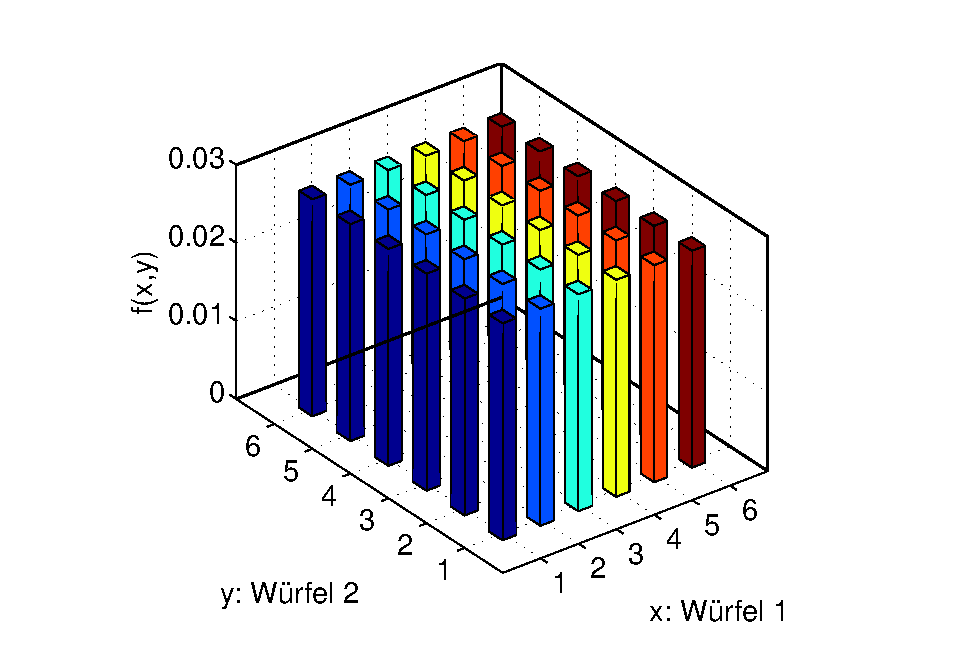
\includegraphics[width=0.5\textwidth]{Kapitel8/Bilder/image1}}
  \caption{Grafische Darstellung der Wahrscheinlichkeitsfunktion f(x,y)}
  \label{fig:Wuerfelexperiment1}
\end{figure}

\noindent Durch Summation der einzelnen Wahrscheinlichkeiten ergibt sich die Verteilungsfunktion F(x,y).

\begin{equation}\label{eq:eightsix}
F(x,y)=\sum _{\xi =1}^{x}\sum _{\psi =1}^{y}f(\xi ,\psi)
\end{equation}

\noindent Sie ist in Bild \ref{fig:Wuerfelexperiment2} dargestellt. 

\noindent 
\begin{figure}[H]
  \centerline{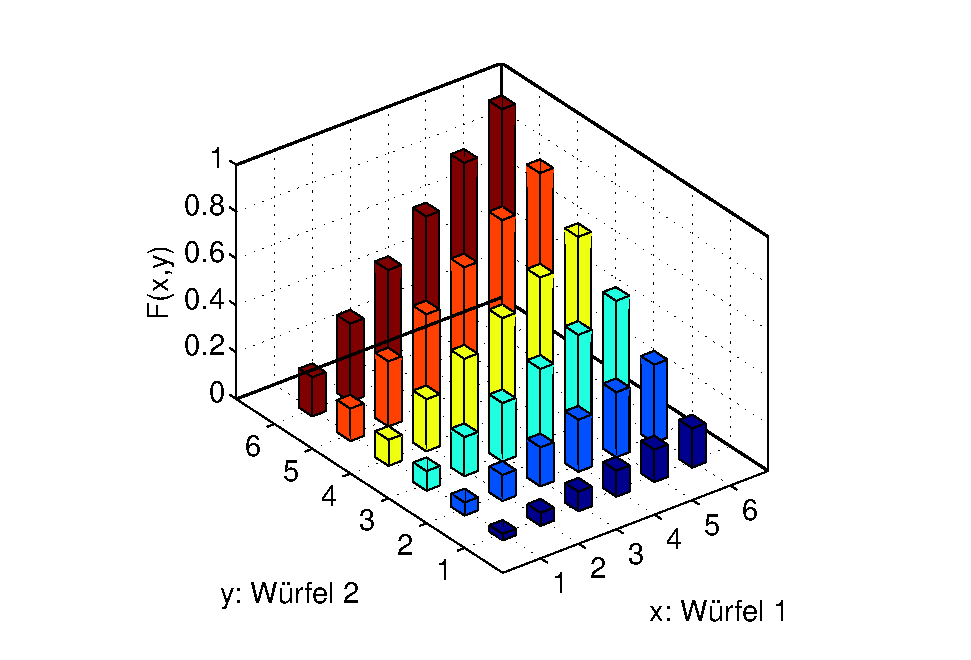
\includegraphics[width=0.5\textwidth]{Kapitel8/Bilder/image2}}
  \caption{Grafische Darstellung der Verteilungsfunktion F(x,y)}
  \label{fig:Wuerfelexperiment2}
\end{figure}

\noindent Die Verteilungsfunktion wird ben\"{o}tigt, um zum Beispiel die Frage zu beantworten, mit welcher Wahrscheinlichkeit beim ersten W\"{u}rfel eine Zahl kleiner gleich 2 und beim zweiten W\"{u}rfel eine Zahl kleiner gleich 4 gew\"{u}rfelt wird. Die Wahrscheinlichkeit hierf\"{u}r ergibt sich aus Gleichung \eqref{eq:eightsix} zu

\begin{equation}\label{eq:eightseven}
F\left(x\le 4,y\le 2\right)=\sum _{x_{j} =1}^{4}\sum _{y_{k} =1}^{2}f\left(x_{j} ,y_{k} \right)  =\dfrac{2\cdot 4}{36} =22\%
\end{equation}

\noindent Das Ergebnis deckt sich mit dem Wert, der aus dem Diagramm in Bild \ref{fig:Wuerfelexperiment2} entnommen werden kann. 

\subsubsection{Stetige Verteilungen}

\noindent Ein Zufallsvektor \underbar{x} hei{\ss}t stetig, wenn es eine Dichtefunktion

\begin{equation}\label{eq:eighteight}
f(\underline{x})=f(x_{1} ,...,x_{M})\ge 0
\end{equation}

\noindent mit der Verteilungsfunktion

\begin{equation}\label{eq:eightnine}
F(\underline{x})=F(x_{1} ,...,x_{M})=\int\limits _{-\infty}^{x_{M}}...\int\limits _{-\infty}^{x_{1}}f(\xi _{1} ,...,\xi _{M}) d\xi _{1} ...d\xi _{M} =\int\limits_{-\infty}^{\underline{x}}f(\underline{\xi}) d\underline{\xi}
\end{equation}

\noindent gibt. Dabei muss f(\underbar{x}) in der ganzen Ebene definiert, nicht negativ und beschr\"{a}nkt sein. Die zu einem Bereich $a_{1} < x_{1} \le b_{1}$ ,{\dots}, $a_{M} < x_{M} \le b_{M}$ geh\"{o}rige Wahrscheinlichkeit ist dann durch

\begin{equation}\label{eq:eightten}
P(a_{1} <x_{1} \le  b_{ 1} ,\, \, ...,\, \,  a_{M} <x_{M} \le b_{M})=\int\limits _{a_{M}}^{b_{M}}...\int\limits _{a_{1}}^{b_{1}}f(\xi _{1} ,...,\xi _{M}) d\xi _{1} ...d\xi _{M}
\end{equation}

\noindent gegeben.\bigskip

\noindent
\colorbox{lightgray}{%
\arrayrulecolor{white}%
\renewcommand\arraystretch{0.6}%
\begin{tabular}{ wl{16.5cm} }
{\fontfamily{phv}\selectfont
\noindent{Beispiel: Fertigung von Passstiften}}
\end{tabular}%
}\medskip

\noindent Die stetige multivariate Verteilung soll anhand eines Beispiels verdeutlicht werden. Hierzu wird die Fertigung von Passstiften in einer automatisierten Fertigungseinrichtung betrachtet. Die Passstifte werden durch ihren Durchmesser D und ihre L\"{a}nge L definiert. Die Fertigung ist auf einen Sollwert des Durchmessers von D = 5 mm und eine L\"{a}nge von L = 19 mm eingestellt.\newline

\noindent Durch den Verschlei{\ss} des Schneidewerkzeuges variieren die tats\"{a}chlichen Werte der Passstifte in einem Bereich von $\pm 1$  mm um den spezifizierten Sollwert. Durch den gleichm\"{a}{\ss}igen Verschlei{\ss} des Schneidewerkzeugs kann der Durchmesser D und die L\"{a}nge L der gefertigten Passstifte mit einer multivariaten Gleichverteilung beschrieben werden. Jeder Wert in den Intervallen  $4 mm < D \leq 6 mm$  und  $18 mm <  L leq 20 mm$  kommt mit gleicher Wahrscheinlichkeit vor. Es soll ermittelt werden, wie viel Ausschuss die Fertigungseinrichtung liefert, wenn eine Toleranzspanne von $ \pm 5$  \% f\"{u}r den Durchmesser D und die L\"{a}nge L zugelassen wird.\newline

\noindent Entsprechend der Beschreibung der Fertigungseinrichtung wird die Dichteverteilung f(D,L) beschrieben durch

\begin{equation}\label{eq:eighteleven}
f(D,L)=\left\{\begin{array}{l} {\dfrac{1}{(b_{1} -a_{1})\cdot (b_{2} -a_{2})} \quad \text{für} \; a_{1} <D \le b_{1} ,a_{2} <L\le b_{2} } \\ 
{ 0 \quad \text{sonst}} \end{array}\right.
\end{equation}

\noindent Bild \ref{fig:Passstifte1} zeigt die durch Gleichung \eqref{eq:eighteleven} definierte Dichteverteilung f(D,L).

\noindent 
\begin{figure}[H]
  \centerline{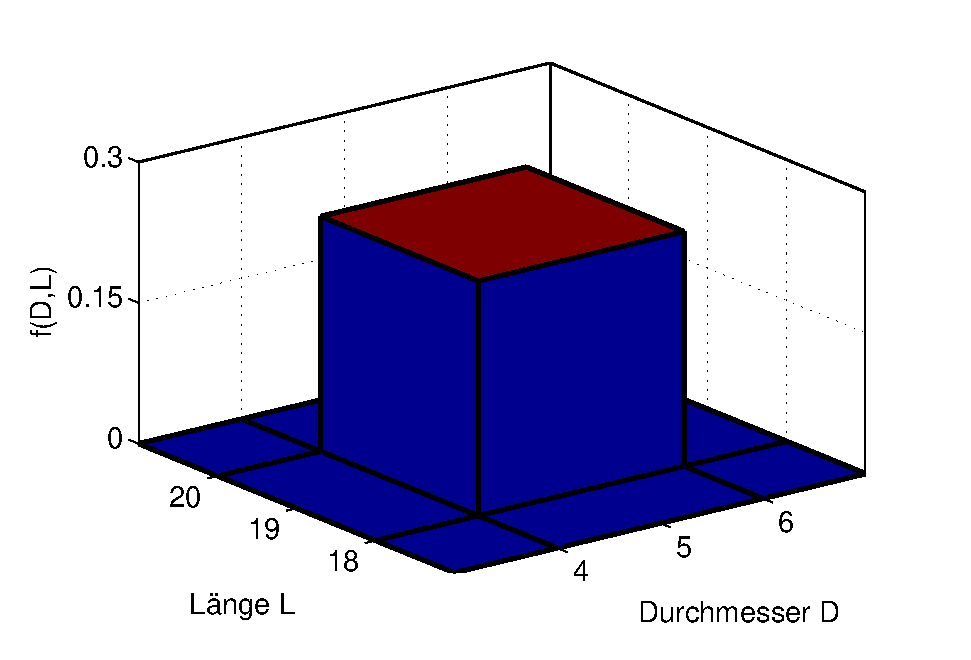
\includegraphics[width=0.5\textwidth]{Kapitel8/Bilder/image3}}
  \caption{Grafische Darstellung der Dichtefunktion f(D,L)}
  \label{fig:Passstifte1}
\end{figure}

\noindent Mit Gleichung \eqref{eq:eightnine} kann die Verteilungsfunktion F(D,L) aufgestellt werden. 

\begin{equation}\label{eq:eighttwelve}
F(D,L)=\int\limits _{18}^{L}\int\limits _{4}^{D}\dfrac{1}{(b_{1} -a_{1})\cdot (b_{2} -a_{2})} d\delta d\lambda =\dfrac{(L-4)\cdot (D-18)}{(6-4)\cdot (20-18)} =\dfrac{(L-4)\cdot (D-18)}{4}
\end{equation}

\noindent Daraus folgt die in Bild \ref{fig:Passstifte2} dargestellte Verteilungsfunktion F(D,L).

\noindent 
\begin{figure}[H]
  \centerline{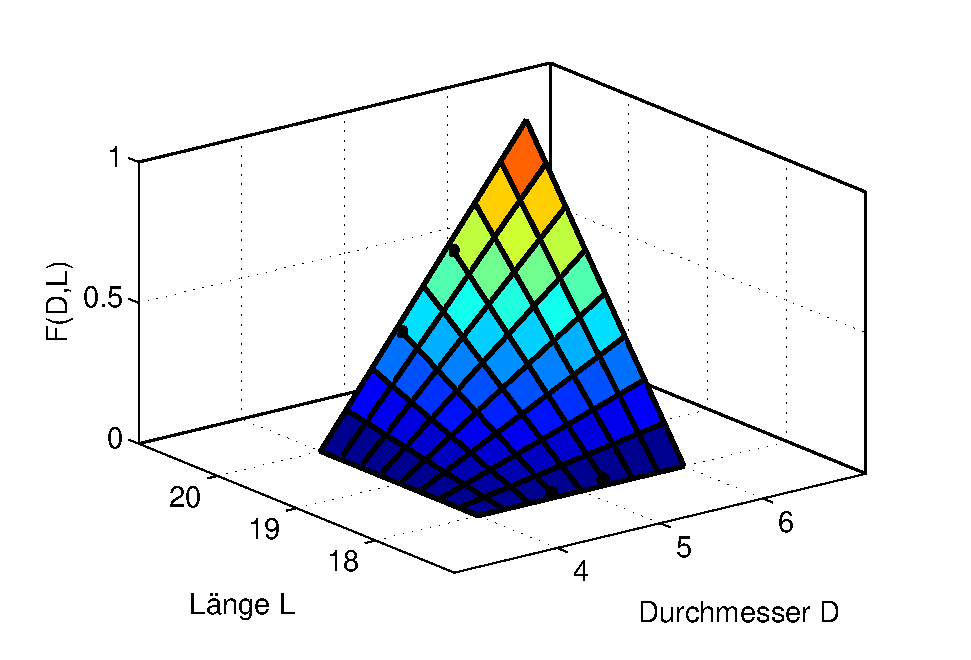
\includegraphics[width=0.5\textwidth]{Kapitel8/Bilder/image4}}
  \caption{Grafische Darstellung der Verteilungsfunktion F(D,L)}
  \label{fig:Passstifte2}
\end{figure}

\noindent Mithilfe der Verteilungsfunktion aus Gleichung \eqref{eq:eighttwelve} wird berechnet, mit welcher Wahrscheinlichkeit P bei der untersuchten Fertigung die produzierten Passstifte in einem spezifizierten Toleranzbereich von $ \pm $ 5 \% um den spezifizierten Durchmessers von D = 5 mm und die spezifizierte L\"{a}nge von L = 19 mm liegen.\newline

\noindent Statt der r\"{a}umlichen Darstellung in Bild \ref{fig:Passstifte2} wird zur Ermittlung der Wahrscheinlichkeit ein Kontur-Plot verwendet, der die Werte die Funktionswerte auf eine Ebene projiziert. Bild \ref{fig:Passstifte3} zeigt die Verteilungsfunktion aus Bild \ref{fig:Passstifte2} als Kontur-Plot.

\noindent 
\begin{figure}[H]
  \centerline{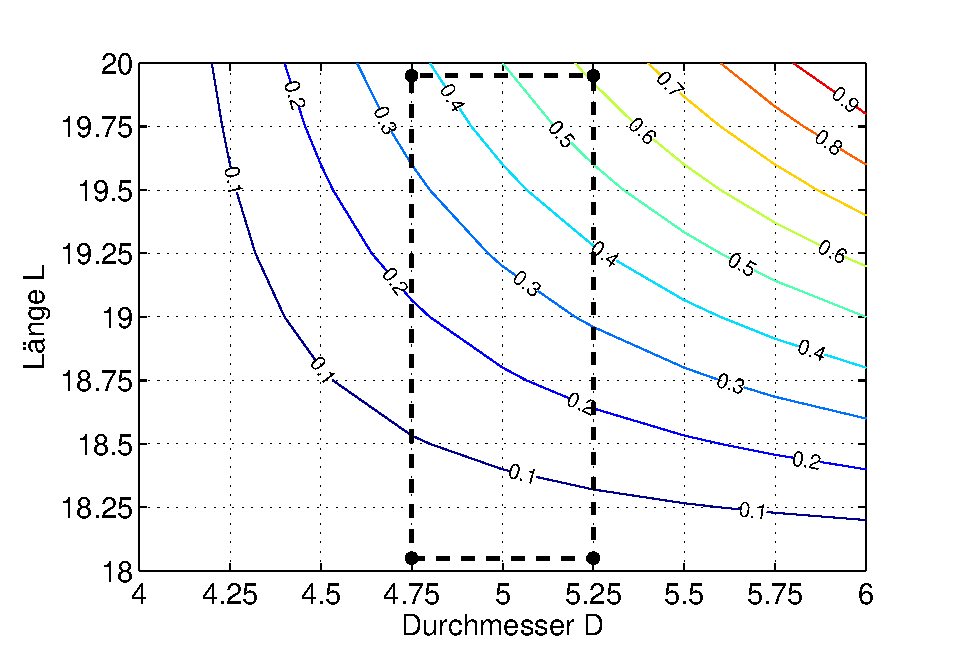
\includegraphics[width=0.5\textwidth]{Kapitel8/Bilder/image5}}
  \caption{Kontur-Plot der Verteilungsfunktion F(D,L)}
  \label{fig:Passstifte3}
\end{figure}

\noindent Die Wahrscheinlichkeit P, mit der die gefertigten Passstifte in dem definierten Toleranzbereich liegen, folgt damit zu

\begin{equation}\label{eq:eightthirteen}
P=F(19.95,5.25)-F(18.05,5.25)-F(19.95,4.75)+F(18.05,4.75)= 23.75\%
\end{equation}

\noindent Daraus ergibt sich ein prozentualer Ausschuss von

\begin{equation}\label{eq:eightfourteen}
A=1-P=1-0.2375=76.25\% 
\end{equation}

\noindent Der Ausschussanteil der Fertigung liegt bei 76.25 \%, lediglich 23.75 \% der gefertigten Passstifte entsprechen den spezifizierten Qualit\"{a}tsanforderungen. 

\subsubsection{Randverteilungen}

\noindent Bei der Auswertung von multivariaten Stichproben werden Randh\"{a}ufigkeiten definiert und ausgerechnet. Dieser Randh\"{a}ufigkeit entspricht bei multivariaten Verteilungen die Randverteilung. Jeder M-dimensionalen Verteilung lassen sich M eindimensionale Randverteilungen zuordnen. Um den Begriff der Randverteilung zu erl\"{a}utern, erfolgt die Betrachtung am Beispiel des W\"{u}rfelns mit zwei unterscheidbaren W\"{u}rfeln aus Abschnitt 8.1.1.\newline

\noindent F\"{u}r das W\"{u}rfelbeispiel wird die Fragestellung untersucht, mit welcher Wahrscheinlichkeit der erste W\"{u}rfel die Zahl 4 aufweist. Der zweite W\"{u}rfel bleibt bei dieser Fragestellung unbeachtet.

\begin{equation}\label{eq:eightfifteen}
f_{x}(4)=P(x=4,y=\text{beliebig})
\end{equation}

\noindent Die Berechnung erfolgt im diskreten Fall durch die Addition aller Wahrscheinlichkeiten f(x,y), bei der das positive Ereignis x = 4 eintritt. 

\begin{equation}\label{eq:eightsixteen}
f_{x}(4)=\sum _{y=1}^{6}f(4,y) =\dfrac{6}{36} =\dfrac{1}{6} =16.7\% 
\end{equation}

\noindent Genauso k\"{o}nnte die Frage nach der Wahrscheinlichkeit gestellt werden, mit der der zweite W\"{u}rfel den Wert 2 aufweist, w\"{a}hrend der erste W\"{u}rfel unber\"{u}cksichtigt bleibt.

\begin{equation}\label{eq:eightseventeen}
f_{y} (2)=P(x=\text{beliebig},y=2) 
\end{equation}

\noindent Die Funktionen aus Gleichung \eqref{eq:eightfifteen} und Gleichung \eqref{eq:eightseventeen} stellen eine eindimensionale Wahrscheinlichkeitsverteilung dar. Sie werden als Randverteilung der Variablen x beziehungsweise y bez\"{u}glich der gegebenen zweidimensionalen Verteilung bezeichnet. Durch Summation ergeben sich die zugeh\"{o}rigen Verteilungsfunktionen der Randverteilungen

\begin{equation}\label{eq:eighteighteen}
F_{x}(x)=P(\xi \le x,y=\text{beliebig})=\sum _{\xi=1}^{x}f_{x} (\xi )
\end{equation}

\noindent und

\begin{equation}\label{eq:eightnineteen}
F_{y} (y)=P(x=\text{beliebig},\psi \le y)=\sum _{\psi =1}^{y}f_{y} (\psi)
\end{equation}

\noindent F\"{u}r das W\"{u}rfelbeispiel aus Abschnitt 8.1.1 ergeben sich die in Tabelle \ref{tab:eightone} aufgelisteten Werte f\"{u}r die Wahrscheinlichkeiten f(x,y) der Wertepaare und die entsprechenden Werte der Randverteilungen.

\begin{table}[H]
\setlength{\arrayrulewidth}{.1em}
\caption{Wahrscheinlichkeitsfunktionen f(x) und f(y) der Randverteilungen}
\setlength{\fboxsep}{0pt}%
\colorbox{lightgray}{%
\arrayrulecolor{white}%
\begin{tabular}{| wc{1.6cm}  wc{1.45cm} | wc{1.45cm} | wc{1.45cm} | wc{1.45cm} | wc{1.45cm} | wc{1.45cm} | wc{1.45cm} | wc{1.45cm} }
\xrowht{10pt}

& & 
\multicolumn{6}{c|}{\fontfamily{phv}\selectfont\textbf{x: Würfel 1}} &
\multirow{2}{*}{\fontfamily{phv}\selectfont\textbf{f$_{y}$(y)}}\\  \xrowht{10pt} 

& & 
\fontfamily{phv}\selectfont\textbf{1} &
\fontfamily{phv}\selectfont\textbf{2} &
\fontfamily{phv}\selectfont\textbf{3} &
\fontfamily{phv}\selectfont\textbf{4} &
\fontfamily{phv}\selectfont\textbf{5} &
\fontfamily{phv}\selectfont\textbf{6} & \\ \hline \xrowht{10pt} 

\multirow{6}{*}{\fontfamily{phv}\selectfont\textbf{y: }}& 
\fontfamily{phv}\selectfont\textbf{1} & 
\fontfamily{phv}\selectfont{1/36} &
\fontfamily{phv}\selectfont{1/36} &
\fontfamily{phv}\selectfont{1/36} &
\fontfamily{phv}\selectfont{1/36} &
\fontfamily{phv}\selectfont{1/36} &
\fontfamily{phv}\selectfont{1/36} & 
\fontfamily{phv}\selectfont{6/36}\\ \cline{2-9} \xrowht{10pt} 

\multirow{6.6}{*}{\fontfamily{phv}\selectfont\textbf{Würfel 2}} & 
\fontfamily{phv}\selectfont\textbf{2} & 
\fontfamily{phv}\selectfont{1/36} &
\fontfamily{phv}\selectfont{1/36} &
\fontfamily{phv}\selectfont{1/36} &
\fontfamily{phv}\selectfont{1/36} &
\fontfamily{phv}\selectfont{1/36} &
\fontfamily{phv}\selectfont{1/36} & 
\fontfamily{phv}\selectfont{6/36}\\ \cline{2-9} \xrowht{10pt} 

& 
\fontfamily{phv}\selectfont\textbf{3} & 
\fontfamily{phv}\selectfont{1/36} &
\fontfamily{phv}\selectfont{1/36} &
\fontfamily{phv}\selectfont{1/36} &
\fontfamily{phv}\selectfont{1/36} &
\fontfamily{phv}\selectfont{1/36} &
\fontfamily{phv}\selectfont{1/36} & 
\fontfamily{phv}\selectfont{6/36}\\ \cline{2-9} \xrowht{10pt} 

& 
\fontfamily{phv}\selectfont\textbf{4} & 
\fontfamily{phv}\selectfont{1/36} &
\fontfamily{phv}\selectfont{1/36} &
\fontfamily{phv}\selectfont{1/36} &
\fontfamily{phv}\selectfont{1/36} &
\fontfamily{phv}\selectfont{1/36} &
\fontfamily{phv}\selectfont{1/36} & 
\fontfamily{phv}\selectfont{6/36}\\ \cline{2-9} \xrowht{10pt} 

& 
\fontfamily{phv}\selectfont\textbf{5} & 
\fontfamily{phv}\selectfont{1/36} &
\fontfamily{phv}\selectfont{1/36} &
\fontfamily{phv}\selectfont{1/36} &
\fontfamily{phv}\selectfont{1/36} &
\fontfamily{phv}\selectfont{1/36} &
\fontfamily{phv}\selectfont{1/36} & 
\fontfamily{phv}\selectfont{6/36}\\ \cline{2-9} \xrowht{10pt} 

& 
\fontfamily{phv}\selectfont\textbf{6} & 
\fontfamily{phv}\selectfont{1/36} &
\fontfamily{phv}\selectfont{1/36} &
\fontfamily{phv}\selectfont{1/36} &
\fontfamily{phv}\selectfont{1/36} &
\fontfamily{phv}\selectfont{1/36} &
\fontfamily{phv}\selectfont{1/36} & 
\fontfamily{phv}\selectfont{6/36}\\ \hline \xrowht{10pt} 

\fontfamily{phv}\selectfont\textbf{f$_{x}$(x)} &
&
\fontfamily{phv}\selectfont{6/36} &
\fontfamily{phv}\selectfont{6/36} &
\fontfamily{phv}\selectfont{6/36} &
\fontfamily{phv}\selectfont{6/36} &
\fontfamily{phv}\selectfont{6/36} &
\fontfamily{phv}\selectfont{6/36} & 
\fontfamily{phv}\selectfont{1}\\ \hline

\end{tabular}%
}\bigskip
\label{tab:eightone}
\end{table}

\noindent Es soll die Frage untersucht werden, mit welcher Wahrscheinlichkeit bei dem ersten W\"{u}rfel eine Zahl kleiner oder gleich 5 gew\"{u}rfelt wird, wenn W\"{u}rfel 2 unber\"{u}cksichtigt bleibt. Diese Wahrscheinlichkeit berechnet sich zu

\begin{equation}\label{eq:eighttwenty}
F_{x} (5)=P(x\le 5,y=\text{beliebig})=\dfrac{6\cdot 5}{36} =83.3\%
\end{equation}

\noindent F\"{u}r den stetigen Fall folgt \"{a}quivalent f\"{u}r die Wahrscheinlichkeitsdichte

\begin{equation}\label{eq:eighttwentyone}
f_{x} (x)=\int\limits _{-\infty}^{\infty}f(x,y) dy
\end{equation}

\noindent und

\begin{equation}\label{eq:eighttwentytwo}
f_{y} (y)=\int\limits _{-\infty }^{\infty }f(x,y) dx
\end{equation}

\noindent Als Bestimmungsgleichung f\"{u}r die Verteilungsfunktion ergeben sich

\begin{equation}\label{eq:eighttwentythree}
F_{x} (x)=\int\limits _{-\infty}^{x}f_{x} (\xi) d\xi
\end{equation}

\noindent und

\begin{equation}\label{eq:eighttwentyfour}
F_{y} (y)=\int\limits _{-\infty }^{y}f_{y} (\psi) d\psi
\end{equation}

\noindent Die Randverteilungen einer stetigen Verteilung sind ebenfalls stetig.\newline

\noindent F\"{u}r den Fall multivariater Datens\"{a}tze mit mehr als zwei Dimensionen ergeben sich M eindimensionale Randverteilungen, die jeweils nur von einer Zufallsvariable abh\"{a}ngen. Mit ihnen k\"{o}nnen oftmals mehrdimensionale Fragestellungen in mehrere univariate Teilprobleme zerlegt werden.

\clearpage

\subsection{Kenngr\"{o}{\ss}en multivariater Wahrscheinlichkeitsverteilungen}

\noindent In der deskriptiven Statistik in Kapitel \ref{seven} werden multivariate Datens\"{a}tze beschrieben. Dazu werden f\"{u}r die vorliegenden Stichproben H\"{a}ufigkeitsverteilungen bestimmt und empirische Kenngr\"{o}{\ss}en berechnet. Im Folgenden werden Verteilungen durch ihren Mittelwert und ihre Kovarianzmatrix beschrieben.

\subsubsection{Arithmetischer Mittelwert als Lagekennwert einer multivariaten Verteilung}

\noindent Die Lage einer mehrdimensionalen Zufallsgr\"{o}{\ss}e \underbar{x} kann \"{u}ber den Vektor der arithmetischen Mittelwerte beschrieben werden. Er ist definiert durch den Erwartungswertvektor von \underbar{x}

\begin{equation}\label{eq:eighttwentyfive}
\underline{\mu }^{T} =E\left(\underline{x}^{T} \right)=\left(\begin{array}{ccc} {E(x_{1})} & {\cdots } & {E(x_{M})} \end{array}\right)=\left(\begin{array}{ccc} {\mu _{1} } & {\cdots } & {\mu _{M}} \end{array}\right)
\end{equation}

\noindent Die Berechnung der einzelnen Mittelwerte erfolgt mit dem in Abschnitt 4.1.3 vorgestellten univariaten Ausdruck f\"{u}r stetige Verteilungen

\begin{equation}\label{eq:eighttwentysix}
\mu =\int\limits _{-\infty}^{\infty}x\cdot f(x) dx
\end{equation}

\noindent Die Mittelwerte $\mu_{m}$ werden \"{u}ber die Randverteilungen $f_{xm}(x_{m})$ der Zufallsvariablen $x_{m}$ bestimmt. Sie sind erwartungsgem\"{a}{\ss} von den \"{u}brigen Variablen $x_{k} \neq x_{m}$ unabh\"{a}ngig. Damit ergibt sich der Mittelwert einer stetigen multivariaten Verteilung zu

\begin{equation}\label{eq:eighttwentyseven}
\underline{\mu}^{T}=E\left(\underline{x}^{T}\right)=\left(\begin{array}{ccc} {\int\limits _{-\infty }^{\infty}x_{1} \cdot f_{x_{1}} (x_{1}) dx_{1} } & {\cdots } & {\int\limits _{-\infty }^{\infty}x_{M} \cdot f_{x_{M}} (x_{ M})\; dx_{M}} \end{array}\right)
\end{equation}

\subsubsection{Kovarianzmatrix als Streuungskennwert einer multivariaten Verteilung}

\noindent Die Streuung einer multivarianten Zufallsgr\"{o}{\ss}e wird \"{u}ber die Kovarianzmatrix bestimmt. Die Kovarianzmatrix ist \"{a}hnlich wie die Varianz bei univariaten Zufallsgr\"{o}{\ss}en \"{u}ber den Erwartungswert definiert.

\begin{equation}\label{eq:eighttwentyeight}
\begin{split}
\Sigma  & = \left(\begin{array}{ccc} {\sigma _{1}^{2} } & {\ldots } & {\sigma _{1M} } \\ {\vdots } & {} & {\vdots } \\ {\sigma _{M1} } & {\cdots } & {\sigma _{M}^{2} } \end{array}\right) \\ 
& = \left(\begin{array}{ccc} {E\left(\left(x_{1} -\mu _{1} \right)^{2} \right)} & {\ldots } & {\sigma _{1M} =E\left(\left(x_{1} -\mu _{1} \right)\cdot \left(x_{M} -\mu _{M} \right)\right)} \\ {\vdots } & {} & {\vdots } \\ {\sigma _{M1} =E\left(\left(x_{M} -\mu _{M} \right)\cdot \left(x_{1} -\mu _{1} \right)\right)} & {\cdots } & {E\left(\left(x_{M} -\mu _{M} \right)^{2} \right)} \end{array}\right) \\ 
& = E\left(\left(X-\left(\begin{array}{c} {1} \\ {\vdots} \\ {1} \end{array}\right)\cdot \underline{\mu }^{T} \right)^{T} \cdot \left(X-\left(\begin{array}{c} {1} \\ {\vdots } \\ {1} \end{array}\right)\cdot \underline{\mu }^{T} \right)\right)
\end{split}
\end{equation}

\noindent Wegen der Kommutativit\"{a}t des Erwartungswertes ist die Kovarianzmatrix symmetrisch zur Hauptdiagonalen. Mit dem arithmetischen Mittelwert und der Kovarianzmatrix ist eine Verteilung hinsichtlich ihrer Lage und Streuung definiert.

\clearpage

\subsection{Unabh\"{a}ngige Zufallsvariablen}

\noindent In vielen F\"{a}llen vereinfacht sich die L\"{o}sung multivariater Aufgabenstellungen, wenn von unabh\"{a}ngigen Zufallsvariablen ausgegangen werden kann. In der Praxis ist dies oftmals zumindest in guter N\"{a}herung gegeben. Aus diesem Grund werden im Folgenden Eigenschaften unabh\"{a}ngiger Variablen n\"{a}her untersucht.

\subsubsection{Verteilungen unabh\"{a}ngiger Zufallsvariablen}

\noindent In Abschnitt 2.4.2 wird die Unabh\"{a}ngigkeit von Ereignissen diskutiert. Es wird gezeigt, dass bei unabh\"{a}ngigen Ereignissen die folgende Beziehung gilt.

\begin{equation}\label{eq:eighttwentynine}
P(A\cap B)=P(A)\cdot P(B)=P(B)\cdot P(A)
\end{equation}

\noindent Auf gleiche Weise kann die Unabh\"{a}ngigkeit bei Zufallsvariablen ausgedr\"{u}ckt werden. Zwei Zufallsvariablen x und y einer zweidimensionalen Verteilung mit der gemeinsamen Verteilungsfunktion F(x,y) sind voneinander unabh\"{a}ngig, wenn f\"{u}r alle m\"{o}glichen Kombinationen von x und y die Beziehung gilt

\begin{equation}\label{eq:eightthirty}
F(x,y)=F_{x} (x)\cdot F_{y} (y)
\end{equation}

\noindent Ist diese Bedingung nicht f\"{u}r alle F\"{a}lle erf\"{u}llt, sind die Zufallsvariablen abh\"{a}ngig. In Analogie zu Gleichung \eqref{eq:eightthirty} kann die Bedingung f\"{u}r die Unabh\"{a}ngigkeit von zwei Variablen nach den Rechenregeln zur Integralrechnung auch durch die Beziehung

\begin{equation}\label{eq:eightthirtyone}
f(x,y)=f_{x} (x)\cdot f_{y} (y)
\end{equation}

\noindent ausgedr\"{u}ckt werden. Dies kann entsprechend auf den multivariaten Fall verallgemeinert werden. Die Bedingung f\"{u}r die Unabh\"{a}ngigkeit kann hierbei durch die Beziehung

\begin{equation}\label{eq:eightthirtytwo}
F(x_{1} ,...,x_{M})=\prod _{m=1}^{M}F_{m} (x_{m})
\end{equation}

\noindent beziehungsweise

\begin{equation}\label{eq:eightthirtythree}
f(x_{1} ,...,x_{M})=\prod _{m=1}^{M}f(x_{m} )
\end{equation}

\noindent bewertet werden.\bigskip

\noindent
\colorbox{lightgray}{%
\arrayrulecolor{white}%
\renewcommand\arraystretch{0.6}%
\begin{tabular}{ wl{16.5cm} }
{\fontfamily{phv}\selectfont
\noindent{Beispiel: Ziehen von verschiedenfarbigen Kugeln}}
\end{tabular}%
}\medskip

\noindent An einem Beispiel soll gepr\"{u}ft werden, ob es sich bei den verwendeten Zufallsvariablen um unabh\"{a}ngige Zufallsvariablen handelt. Hierzu wird angenommen, dass in einer Urne zehn Kugeln liegen. Vier Kugeln haben die Farbe Blau, die restlichen Kugeln sind rot. Es werden nacheinander zwei Kugeln gezogen, die zuerst gezogene Kugel wird nicht zur\"{u}ckgelegt.\newline

\noindent Im Folgenden werden die Zufallsvariablen x und y betrachtet. Die Zufallsvariable x repr\"{a}sentiert die Zahl der blauen Kugeln beim ersten Zug, die Zufallsvariable y die Anzahl blauer Kugeln beim zweiten Zug. Die Werte der Wahrscheinlichkeitsfunktionen k\"{o}nnen anhand der H\"{a}ufigkeiten berechnet werden. Diese sind in Tabelle \ref{tab:eighttwo} zusammengefasst.

\clearpage

\noindent Tabelle 8.2: Wahrscheinlichkeiten des Zufallsexperimentes 
\begin{table}[H]
\setlength{\arrayrulewidth}{.1em}
\caption{Wahrscheinlichkeitsfunktionen f(x) und f(y) der Randverteilungen}
\setlength{\fboxsep}{0pt}%
\colorbox{lightgray}{%
\arrayrulecolor{white}%
\begin{tabular}{| wc{1cm} wc{0.3cm} wc{0.3cm} | wc{6.8cm} | wc{6.8cm} }
\xrowht{20pt}

& & &
\multicolumn{2}{c}{\fontfamily{phv}\selectfont\textbf{Zug 1}}\\  \xrowht{10pt} 

& & &
\fontfamily{phv}\selectfont\textbf{blaue Kugel} &
\fontfamily{phv}\selectfont\textbf{rote Kugel}\\ \xrowht{10pt}

& & &
\fontfamily{phv}\selectfont\textbf{(x = 1)} &
\fontfamily{phv}\selectfont\textbf{(x = 0)}\\ \hline \xrowht{20pt}

\multirow{10}{*}{\fontfamily{phv}\selectfont\textbf{\rotatebox{90}{Zug 2}}}& 
\multirow{2}{*}{\fontfamily{phv}\selectfont\textbf{\rotatebox{90}{blaue Kugel}}} & 
\multirow{5}{*}{\fontfamily{phv}\selectfont\textbf{\rotatebox{90}{(y = 1)}}} &
&
\\ \xrowht{10pt}

& 
& 
&
\fontfamily{phv}\selectfont{$f\left(1,1\right)=\dfrac{4}{10} \cdot \dfrac{3}{9} =\dfrac{2}{15} $} &
\fontfamily{phv}\selectfont{$f\left(0,1\right)=\dfrac{6}{10} \cdot \dfrac{4}{9} =\dfrac{4}{15} $} \\ \xrowht{20pt}

& 
& 
&
&
\\ \cline{2-5} \xrowht{20pt} 
 
& 
\multirow{2}{*}{\fontfamily{phv}\selectfont\textbf{\rotatebox{90}{rote Kugel}}} & 
\multirow{5}{*}{\fontfamily{phv}\selectfont\textbf{\rotatebox{90}{(y = 0)}}}&
&
\\\xrowht{10pt}

& 
& 
&
\fontfamily{phv}\selectfont{$f(1,0)=\dfrac{4}{10} \cdot \dfrac{6}{9} =\dfrac{4}{15} $} &
\fontfamily{phv}\selectfont{$f(0,0)=\dfrac{6}{10} \cdot \dfrac{5}{9} =\dfrac{1}{3} $} \\ \xrowht{20pt}

& 
& 
&
&
\\ \hline

\end{tabular}%
}\bigskip
\label{tab:eighttwo}
\end{table}

\noindent Zur \"{U}berpr\"{u}fung der Unabh\"{a}ngigkeit m\"{u}ssen die Werte der Randverteilungen berechnet werden. Die Wahrscheinlichkeit, dass beim ersten Zug keine blaue Kugel gezogen wird, berechnet sich zu

\begin{equation}\label{eq:eightthirtyfour}
f_{x} (x=0)=\dfrac{4}{15} +\dfrac{1}{3} =0.6
\end{equation}


\noindent und die Wahrscheinlichkeit, dass beim zweiten Zug keine blaue Kugel gezogen wird, ergibt sich zu

\begin{equation}\label{eq:eightthirtyfive}
f_{y} (y=0)=\dfrac{4}{15} +\dfrac{1}{3} =0.6
\end{equation}

\noindent Damit ergibt sich bei unabh\"{a}ngigen Zufallsvariablen die Wahrscheinlichkeit, zweimal hintereinander eine rote Kugel zu ziehen, durch die Multiplikation der Wahrscheinlichkeiten der Randverteilungen aus Gleichung \eqref{eq:eightthirtyfour} und Gleichung \eqref{eq:eightthirtyfive} zu

\begin{equation}\label{eq:eightthirtysix}
f_{x} (x=0)\cdot f_{y} (y=0)=0.6\cdot 0.6=0.36
\end{equation}

\noindent Der Vergleich mit Tabelle \ref{tab:fourfour} zeigt, dass die Wahrscheinlichkeit f\"{u}r dieses Ereignis 0.33 betr\"{a}gt. Damit gilt zumindest f\"{u}r ein Wertepaar die Beziehung

\begin{equation}\label{eq:eightthirtyseven}
f(x,y)\ne f_{x} (x)\cdot f_{y} (y)
\end{equation}

\noindent Die Variablen sind demnach abh\"{a}ngig. Die Ursache liegt darin, dass die Wahrscheinlichkeit, beim zweiten Zug eine blaue Kugel zu ziehen, durch den ersten Zug ver\"{a}ndert wird. W\"{u}rde die Kugel des ersten Zuges zur\"{u}ck in die Urne gelegt, g\"{a}be es keine Ver\"{a}nderung der Wahrscheinlichkeit gegen\"{u}ber der Ausgangsposition. Die Zufallsgr\"{o}{\ss}en w\"{a}ren in diesem Fall unabh\"{a}ngig.

\subsubsection{Kovarianz unabh\"{a}ngiger Zufallsvariablen}

\noindent Handelt es sich bei den Zufallsvariablen x und y um unabh\"{a}ngige Zufallsvariablen, gilt f\"{u}r deren Kovarianz $\sigma_{xy}$

\begin{equation}\label{eq:eightthirtyeight}
\sigma _{xy} =E\left((x-\mu _{x})\cdot (y-\mu _{y})\right)=0
\end{equation}

\noindent Um diese Beziehung zu beweisen, muss Gleichung \eqref{eq:eightthirtyeight} weiter umgeformt werden. Ausmultiplizieren des Terms f\"{u}hrt zu

\begin{equation}\label{eq:eightthirtynine}
\begin{split}
\sigma _{xy} & = E(x\cdot y)-E(x)\cdot \mu _{y} -E(y)\cdot \mu _{x} +\mu _{x} \cdot \mu _{y} =E(x\cdot y)-\mu _{x} \cdot \mu _{y} -\mu _{x} \cdot \mu _{y} +\mu _{x} \cdot \mu _{y}\\
& = E(x\cdot y)-\mu _{x} \cdot \mu _{y}= E(x\cdot y)-E(x)\cdot E(y) = 0
\end{split}
\end{equation}

\noindent Damit die Kovarianz der Zufallsvariablen x und y zu null wird, muss demnach gelten

\begin{equation}\label{eq:eightfourty}
E(x\cdot y)=E(x)\cdot E(y)
\end{equation}

\noindent Diese Bedingung wird f\"{u}r diskrete und stetige Zufallsvariable berechnet. Aus Kapitel 4 ist bekannt, dass sich der Erwartungswert f\"{u}r eine diskrete Zufallsvariable z berechnet aus

\begin{equation}\label{eq:eightfourtyone}
E(z)=\sum _{j=-\infty }^{\infty}z_{j}  \cdot f(z_{j})=\sum _{j=-\infty }^{\infty }z_{j}  \cdot P(z=z_{j})
\end{equation}

\noindent Wird die Zufallsvariable z aus Gleichung \eqref{eq:eightfourtyone} durch das Produkt der Zufallsvariablen x und y ersetzt, ergibt sich

\begin{equation}\label{eq:eightfourtytwo}
E(x\cdot y)=\sum _{j=-\infty }^{\infty }\sum _{k=-\infty}^{\infty}x_{j}  \cdot y_{k} \cdot f\left(x_{j} ,y_{k} \right) =\sum _{j=-\infty }^{\infty}\sum _{k=-\infty}^{\infty}x_{j}  \cdot y_{k} \cdot P(x=x_{j} \cap y=y_{k})
\end{equation}

\noindent Da es sich bei den Zufallsvariablen x und y um unabh\"{a}ngige Zufallsgr\"{o}{\ss}en handelt, kann mit Gleichung \eqref{eq:twosixtyfive} die vorige Gleichung \eqref{eq:eightfourtytwo} umgestellt werden zu

\begin{equation}\label{eq:eightfourtythree}
\begin{split}
E(x\cdot y) & = \sum _{j=-\infty}^{\infty}\sum _{k=-\infty }^{\infty }x_{j}  \cdot y_{k} \cdot P\left(x=x_{j} \cap y=y_{k} \right) =\sum _{j=-\infty}^{\infty}x_{j}  \cdot P(x=x_{j})\cdot \sum _{j=-\infty}^{\infty}y_{k}  \cdot P(y=y_{k} ) \\ 
& = \sum _{j=-\infty}^{\infty}x_{j}  \cdot f_{x_{j}} \left(x_{j} \right)\cdot \sum _{j=-\infty}^{\infty}y_{k}  \cdot f_{x_{k}} (x_{k})=E(x)\cdot E(y)
\end{split}
\end{equation}

\noindent Die Umrechnung hat gezeigt, dass die Beziehung aus Gleichung \eqref{eq:eightfourty} f\"{u}r unabh\"{a}ngige diskrete Zufallsvariablen erf\"{u}llt ist und damit die Kovarianz zu Null wird. Analog kann dies mit den Regeln zum Erwartungswert aus Kapitel 4 und unter Ber\"{u}cksichtigung von Gleichung \eqref{eq:eightthirtyone} auch f\"{u}r stetige Zufallsvariablen gezeigt werden.

\begin{equation}\label{eq:eightfourtyfour}
\begin{split}
E(x\cdot y) & =\int\limits _{-\infty}^{\infty}z\cdot f(z)  dz=\int\limits _{-\infty}^{\infty}\int\limits _{-\infty }^{\infty}x\cdot y\cdot f(x,y) dxdy=\int\limits _{-\infty }^{\infty}\int\limits _{-\infty}^{\infty}x\cdot y\cdot f_{x} (x)\cdot f_{y} \left(y\right) dxdy \\ 
& = \int\limits _{-\infty}^{\infty}x\cdot f_{x} (x)  dx\cdot \int\limits _{-\infty}^{\infty}y\cdot f_{y} (y)  dy=E(x)\cdot E(y)
\end{split}
\end{equation}

\noindent Damit gilt allgemein, dass die Kovarianz unabh\"{a}ngiger Zufallsgr\"{o}{\ss}en null ist.

\clearpage

\subsection{Funktionen von Zufallsvariablen}

\noindent Zur Beschreibung von Zufallsexperimenten kann es notwendig sein, eine Funktion von Zufallsvariablen abzubilden. Dabei wird jedem m\"{o}glichen Wert des Vektors von Zufallsvariablen \underbar{x} \"{u}ber die Funktion g(\underbar{x}) ein reeller Wert zugeordnet. Hierbei sind vier grundlegende Rechenoperationen von Bedeutung, mit denen komplexe Funktionen analysiert werden k\"{o}nnen:

\begin{enumerate}
    \item Summe von Zufallszahlen
    \item Differenz von Zufallszahlen
    \item Produkt von Zufallszahlen
    \item Quotient von Zufallszahlen
\end{enumerate}

\noindent Die Herleitung beschr\"{a}nkt sich der \"{U}bersicht wegen auf zwei stetige Zufallsvariablen. Au{\ss}erdem wird an dieser Stelle der Zusammenhang f\"{u}r die Summe von Zufallszahlen hergeleitet. Die Herleitungen zu den \"{u}brigen Rechenoperationen sind \"{a}hnlich. Die dabei erlangten Erkenntnisse lassen sich auf Funktionen diskreter Zufallsvariablen und auch auf mehrere Zufallsvariablen erweitern. 

\subsubsection{Summe von Zufallsvariablen}

\noindent Im Folgenden soll die Summenfunktion der unabh\"{a}ngigen Zufallsvariablen x und y untersucht werden. Die Verteilungsfunktion der neuen Zufallsvariablen der Form

\begin{equation}\label{eq:eightfourtyfive}
z=x+y
\end{equation}

\noindent berechnet sich zu

\begin{equation}\label{eq:eightfourtysix}
P(\zeta \le z)=F_{z} (z)= \iint\limits_{x+y\le z}f(x,y) dxdy
\end{equation}

{\fontfamily{phv}\selectfont
\noindent\textbf{Wahrscheinlichkeitsdichte der Summe von unabh\"{a}ngigen Zufallszahlen}}\smallskip

\noindent Wie bereits bei der linearen Transformation muss zur Umformung des Integrals eine entsprechende Koordinatentransformation durchgef\"{u}hrt werden. Hierbei wird

\begin{equation}\label{eq:eightfourtyseven}
y=z-x
\end{equation}

\noindent gesetzt. Diese Koordinatentransformation erfordert eine Umrechnung des Integranden. Sie l\"{a}sst sich nach dem Transformationssatz durch die Berechnung der Jacobi-Determinanten durchf\"{u}hren. Es ergibt sich 

\begin{equation}\label{eq:eightfourtyeight}
dxdy=\left|\left(\begin{array}{cc} {\dfrac{\partial x}{\partial x}} & {\dfrac{\partial x}{\partial z}} \\ {\dfrac{\partial y}{\partial x}} & {\dfrac{\partial y}{\partial y}} \end{array}\right)\right|dxdz=\left|\left(\begin{array}{cc} {\dfrac{\partial x}{\partial x}} & {\dfrac{\partial x}{\partial z}} \\ {\dfrac{\partial (z-x)}{\partial x}} & {\dfrac{\partial (z-x)}{\partial z} } \end{array}\right)\right|dxdz=\left|\left(\begin{array}{cc} {1} & {0} \\ {-1} & {1} \end{array}\right)\right|dxdz=\left|1\right|dxdz
\end{equation}

\noindent Damit folgt Gleichung \eqref{eq:eightfourtysix} zu

\begin{equation}\label{eq:eightfourtynine}
F_{z} (z)=\int\limits _{-\infty}^{z}\int\limits _{-\infty}^{\infty}f(x,\zeta -x) dxd\zeta =\int\limits _{-\infty}^{z}f_{z} (\zeta ) d\zeta
\end{equation}

\noindent Die Wahrscheinlichkeitsdichte ergibt sich aus dem inneren Integral zu

\begin{equation}\label{eq:eightfifty}
f_{z} (z)=\int\limits _{-\infty}^{\infty}f(x,z-x) dx
\end{equation}

\noindent Im Fall unabh\"{a}ngiger Zufallsvariablen kann sie als Produkt zweier Wahrscheinlichkeitsdichten dargestellt werden. Das Integral entspricht in diesem Fall der Faltung der Wahrscheinlichkeitsdichten.

\begin{equation}\label{eq:eightfiftyone}
f_{z} (z)=\int\limits _{-\infty}^{\infty}f(x,z-x) dx =\int\limits _{-\infty}^{\infty}f_{x} (x)\cdot f_{y} (z-x) dx =f_{x} (x)*f_{y} (z-x)
\end{equation}

\noindent Diese Erkenntnis kann auf M unabh\"{a}ngige Zufallsvariablen erweitert werden. Die Verteilungsfunktion der Summe von M unabh\"{a}ngigen Zufallsvariablen

\begin{equation}\label{eq:eightfiftytwo}
z=\sum _{m=1}^{M}x_{m}
\end{equation}

\noindent ergibt sich aus der Faltung der M Verteilungsfunktionen $f_{xm}(x_{m})$.\bigskip

{\fontfamily{phv}\selectfont
\noindent\textbf{Kenngr\"{o}{\ss}en f\"{u}r die Summe von Zufallsvariablen}}\smallskip

\noindent Zur Berechnung des Mittelwertes $\mu_{z}$ wird die Definition \"{u}ber den Erwartungswert herangezogen. Mit der Linearit\"{a}t des Erwartungswert-Operators folgt 

\begin{equation}\label{eq:eightfiftythree}
\mu _{z} =E(z)=E(x+y)=E(x)+E(y)=\mu _{x} +\mu _{y}
\end{equation}

\noindent Der Gesamtmittelwert setzt sich nach Gleichung \eqref{eq:eightfiftythree} aus der Summe der Einzelmittelwerte zusammen. Nach den Rechenregeln zum Erwartungswert errechnet sich die Varianz einer Zufallsvariable z zu

\begin{equation}\label{eq:eightfiftyfour}
\sigma _{z}^{2} =E(z^{2})-E(z)^{2}
\end{equation}

\noindent Mit z als Summe der Zufallsvariablen x und y ergibt sich

\begin{equation}\label{eq:eightfiftyfive}
E(z^{2})=E\left(x^{2} +2\cdot x\cdot y+y^{2} \right)=E\left(x^{2} \right)+2\cdot E(x\cdot y)+E\left(y^{2} \right)
\end{equation}

\noindent und

\begin{equation}\label{eq:eightfiftysix}
\left(E(z)\right)^{2} =\left(E(x+y)\right)^{2} =\left(E(x)+E(y)\right)^{2} =\left(E(x)\right)^{2} +2\cdot E(x)\cdot E(y)+\left(E(y)\right)^{2}
\end{equation}

\noindent Werden die beiden Ausdr\"{u}cke aus Gleichung \eqref{eq:eightfiftyfive} und Gleichung \eqref{eq:eightfiftysix} in die Gleichung \eqref{eq:eightfiftyfour} der Varianz $\sigma_{z}^{2}$ eingesetzt, ergibt sich

\begin{equation}\label{eq:eightfiftyseven}
\sigma _{z}^{2} =\left(E\left(x^{2} \right)-\left(E(x)\right)^{2} \right)+\left(E\left(y^{2} \right)-\left(E(y)\right)^{2} \right)+2\cdot \left(E\left(x\cdot y\right)-E(x)\cdot E(y)\right)
\end{equation}

\noindent In den ersten Klammern der Gleichung stehen die Varianzen der Zufallsvariablen x und y. Der letzte Ausdruck kann zusammengefasst dargestellt werden als

\begin{equation}\label{eq:eightfiftyeight}
E(x\cdot y)-E(x)\cdot E(y)=\sigma _{xy}
\end{equation}

\noindent Die Varianz der Summe zweier Zufallsvariablen ergibt sich damit allgemein zu

\begin{equation}\label{eq:eightfiftynine}
\sigma _{z}^{2} =\sigma _{x}^{2} +\sigma _{y}^{2} +2\cdot \sigma _{xy}
\end{equation}

\noindent Die Gr\"{o}{\ss}e $\sigma_{xy}$ ist die Kovarianz der Zufallsvariablen x und y. \newline

\noindent Sind die Variablen x und y unabh\"{a}ngig voneinander, ist die Kovarianz null. Damit ergibt sich die Varianz der Summe unabh\"{a}ngiger Zufallsvariablen x und y aus der Summe 

\begin{equation}\label{eq:eightsixty}
\sigma _{z}^{2} =\sigma _{x}^{2} +\sigma _{y}^{2}
\end{equation}

\noindent Diese Regeln kann auf M unabh\"{a}ngige Zufallsvariablen $x_{m}$ mit den Mittelwerten $\mu_{m}$ und $\sigma_{m}$ erweitert werden. Die Summe der Zufallsvariablen

\begin{equation}\label{eq:eightsixtyone}
z=\sum _{m=1}^{M}x_{m}
\end{equation}

\noindent besitzt demzufolge einen Mittelwert bei

\begin{equation}\label{eq:eightsixtytwo}
\mu _{z} =\sum _{m=1}^{M}\mu _{m}
\end{equation}

\noindent und weist eine Varianz von

\begin{equation}\label{eq:eightsixtythree}
\sigma _{z}^{2} =\sum _{m=1}^{M}\sigma _{m}^{2}
\end{equation}

\noindent auf. 

\subsubsection{Zusammenfassung Funktionen von Zufallszahlen}

\noindent Analog zu der Herleitung f\"{u}r die Summe zweier Zufallszahlen kann bei den \"{u}brigen Rechenoperationen vorgegangen werden. Hierzu muss zun\"{a}chst eine entsprechende Zufallsvariable definiert werden. Durch eine Variablentransformation ergibt sich die Verteilungsfunktion der neuen Zufallsvariable z. Mithilfe des Erwartungswertoperators lassen sich Ausdr\"{u}cke f\"{u}r den Mittelwert $\mu_{z}$ und der Varianz $\sigma_{z}^{2}$ berechnen. F\"{u}r unabh\"{a}ngige Zufallsvariable sind in Tabelle \ref{tab:eightthree} die Dichtefunktion f(z), der Mittelwert $\mu_{z}$ und die Varianz $\sigma_{z}^{2}$ der verschiedenen Rechenoperationen zusammengestellt. 

\clearpage

\begin{table}[H]
\setlength{\arrayrulewidth}{.1em}
\caption{Zusammenfassung der Funktionen von unabh\"{a}ngigen Zufallsvariablen}
\setlength{\fboxsep}{0pt}%
\colorbox{lightgray}{%
\arrayrulecolor{white}%
\begin{tabular}{ wc{3cm} | wc{5.6cm} | wc{3cm} | wc{4cm} }
\hline\xrowht{10pt}

\fontfamily{phv}\selectfont\textbf{Rechenoperation} &
\fontfamily{phv}\selectfont\textbf{Dichtefunktion f(z)} &
\fontfamily{phv}\selectfont\textbf{Mittelwert µ$_{z}$} &
\fontfamily{phv}\selectfont\textbf{Varianz $\sigma_{z}^{2}$}\\ \hline \xrowht{25pt}

\fontfamily{phv}\selectfont\textbf{Addition} & 
\fontfamily{phv}\selectfont{$f_{x+y}(z)=\int\limits _{-\infty}^{\infty}f_{x} (x)\cdot f_{y} (z-x)dx $} &
\fontfamily{phv}\selectfont{$\mu _{z} =\mu _{x} +\mu _{y}$} & 
\fontfamily{phv}\selectfont{$\sigma _{z}^{2} =\sigma _{x}^{2} +\sigma _{y}^{2}$} \\ \hline\xrowht{25pt}

\fontfamily{phv}\selectfont\textbf{Subtraktion} & 
\fontfamily{phv}\selectfont{$f_{x-y} (z)=\int\limits _{-\infty}^{\infty}f_{x}(x)\cdot f_{y}(x-z)dx$} &
\fontfamily{phv}\selectfont{$\mu _{z} =\mu _{x} -\mu _{y}$} & 
\fontfamily{phv}\selectfont{$\sigma _{z}^{2} =\sigma _{x}^{2} +\sigma _{y}^{2} $} \\ \hline\xrowht{25pt}

\fontfamily{phv}\selectfont\textbf{Multiplikation} & 
\fontfamily{phv}\selectfont{$f_{x\cdot y} (z)=\int\limits _{-\infty}^{\infty}\left|\dfrac{1}{x} \right|\cdot f_{x} (x)\cdot f_{y} \left(\dfrac{z}{x} \right)dx $} &
\fontfamily{phv}\selectfont{$\mu _{z} =\mu _{x} \cdot \mu _{y} $} & 
\fontfamily{phv}\selectfont{$\sigma _{z}^{2} =\mu _{x}^{2} \cdot \sigma _{y}^{2} +\mu _{y}^{2} \cdot \sigma _{x}^{2}$} \\ \hline\xrowht{25pt}

\fontfamily{phv}\selectfont\textbf{Division} & 
\fontfamily{phv}\selectfont{$f_{x/y} (z)=\int\limits _{-\infty}^{\infty}\left|\dfrac{x}{z^{2}} \right|\cdot f_{x} (x)\cdot f_{y} \left(\dfrac{x}{z} \right)dx $} &
\fontfamily{phv}\selectfont{$\mu _{z} =\mu _{{}^{{}_{x} } } \cdot \mu _{1/y} $} & 
\fontfamily{phv}\selectfont{$\sigma _{z}^{2} =\mu _{x}^{2} \cdot \sigma _{1/y}^{2} +\mu _{1/y}^{2} \cdot \sigma _{x}^{2} $} \\ \hline

\end{tabular}%
}
\label{tab:eightthree}
\end{table}

\noindent Die in diesem Kapitel vorgestellten Funktionen zweier unabh\"{a}ngiger Zufallszahlen lassen sich durch wiederholte Anwendung auf Funktionen mehrerer Zufallsvariablen erweitern.\newline

\noindent Im Fall abh\"{a}ngiger Zufallsvariablen kann die Dichtefunktion nicht auf diese Art berechnet werden. Die Rechenregeln f\"{u}r Mittelwert und Standardabweichung bleiben jedoch f\"{u}r die Summe und die Differenz von Zufallsvariablen erhalten, und es ergeben sich die in Tabelle \ref{tab:eightfour}dargestellten Zusammenh\"{a}nge. \newline

\begin{table}[H]
\setlength{\arrayrulewidth}{.1em}
\caption{Zusammenfassung der Funktionen von abh\"{a}ngigen Zufallsvariablen}
\setlength{\fboxsep}{0pt}%
\colorbox{lightgray}{%
\arrayrulecolor{white}%
\begin{tabular}{ wc{5.3cm} | wc{5.3cm} | wc{5.3cm} }
\hline\xrowht{10pt}

\fontfamily{phv}\selectfont\textbf{Rechenoperation} &
\fontfamily{phv}\selectfont\textbf{Mittelwert µ$_{z}$} &
\fontfamily{phv}\selectfont\textbf{Varianz $\sigma_{z}^{2}$}\\ \hline \xrowht{25pt}

\fontfamily{phv}\selectfont\textbf{Addition} & 
\fontfamily{phv}\selectfont{$\mu _{z} =\mu _{x} +\mu _{y}$} &
\fontfamily{phv}\selectfont{$\sigma _{z}^{2} =\sigma _{x}^{2} +\sigma _{y}^{2} +2\cdot \sigma _{xy} $} \\ \hline\xrowht{25pt}

\fontfamily{phv}\selectfont\textbf{Subtraktion} & 
\fontfamily{phv}\selectfont{$\mu _{z} =\mu _{x} -\mu _{y}$} & 
\fontfamily{phv}\selectfont{$\sigma _{z}^{2} =\sigma _{x}^{2} +\sigma _{y}^{2} -2\cdot \sigma _{xy}$} \\ \hline

\end{tabular}%
}
\label{tab:eightfour}
\end{table}

\noindent Durch Anwenden dieser Funktionen l\"{a}sst sich eine multivariate Fragestellung auf eine univariate Fragestellung abbilden. Sie sind insbesondere bei der Toleranzrechnung von Bedeutung.

\clearpage

\subsection{Zentraler Grenzwertsatz}

\noindent Nach dem zentralen Grenzwertsatz besitzt eine Zufallsvariable, die sich aus der Summe von unabh\"{a}ngigen Zufallsvariablen ergibt, eine Normalverteilung. Zum Beweis wird von den Zufallsvariablen $x_{1}$, ..., $x_{M}$ ausgegangen, die alle denselben Mittelwert µ und dieselbe Varianz $\sigma^{2}$ aufweisen. Die Zufallsvariable y, die sich aus der Summe unabh\"{a}ngiger Zufallsvariablen ergibt

\begin{equation}\label{eq:eightsixtyfour}
y=x_{1} +x_{2} +...+x_{M} =\sum _{m=1}^{M}x_{m}
\end{equation}

\noindent hat nach Gleichung \eqref{eq:eightsixtytwo} den Mittelwert µ${}_{y} = M\cdot\mu$ und nach Gleichung \eqref{eq:eightsixtythree} die Varianz $\sigma_{y}^{2}= M\cdot \sigma^{2}$. Sind die Variablen $x_{1}$, ..., $x_{M}$ normalverteilt, ist auch die Variable y normalverteilt und die Zufallsvariable 

\begin{equation}\label{eq:eightsixtyfive}
z=\dfrac{y-\mu _{y}}{\sigma _{y}} =\dfrac{y-M\cdot \mu}{\sigma \cdot \sqrt{M}}
\end{equation}

\noindent weist eine Standardnormalverteilung auf.\newline

\noindent Sind die Variablen nicht normalverteilt, so ist die Zufallsvariable z aus Gleichung \eqref{eq:eightsixtyfive} f\"{u}r eine gro{\ss}e Anzahl M von Summanden asymptotisch standardnormalverteilt. Diese wichtige Beziehung wird als zentraler Grenzwertsatz der Wahrscheinlichkeitsrechnung bezeichnet. Er ist der wesentliche Grund f\"{u}r die gro{\ss}e Bedeutung der Normalverteilung in der Wahrscheinlichkeitstheorie. Statt eines Beweises wird der zentrale Grenzwertsatz grafisch motiviert. Als Basis werden Variablen $x_{m}$ mit einer Gleichverteilung in einem Bereich von - 0.2 {\dots} 0.2 verwendet. Sie besitzen eine Gleichverteilung mit einem Mittelwert µ = 0 und einer Varianz $\sigma^{2} = 0.0133$. Die Wahrscheinlichkeitsverteilung der Summe von unabh\"{a}ngigen Zufallsvariablen ergibt sich nach Gleichung \eqref{eq:eightfiftyone} aus der Faltung der einzelnen Wahrscheinlichkeitsdichten.

\begin{equation}\label{eq:eightsixtysix}
f(y)=f(x_{1})*f(x_{2})*...*f(x_{M})
\end{equation}

\noindent Die Wahrscheinlichkeitsdichte f(y) h\"{a}ngt davon ab, wie viele Faltungen stattgefunden haben. Bild \ref{fig:Grenzwertsatz1} stellt die Wahrscheinlichkeitsdichten f\"{u}r unterschiedliche Anzahlen M von Zufallsvariablen dar.

\noindent 
\begin{figure}[H]
  \centerline{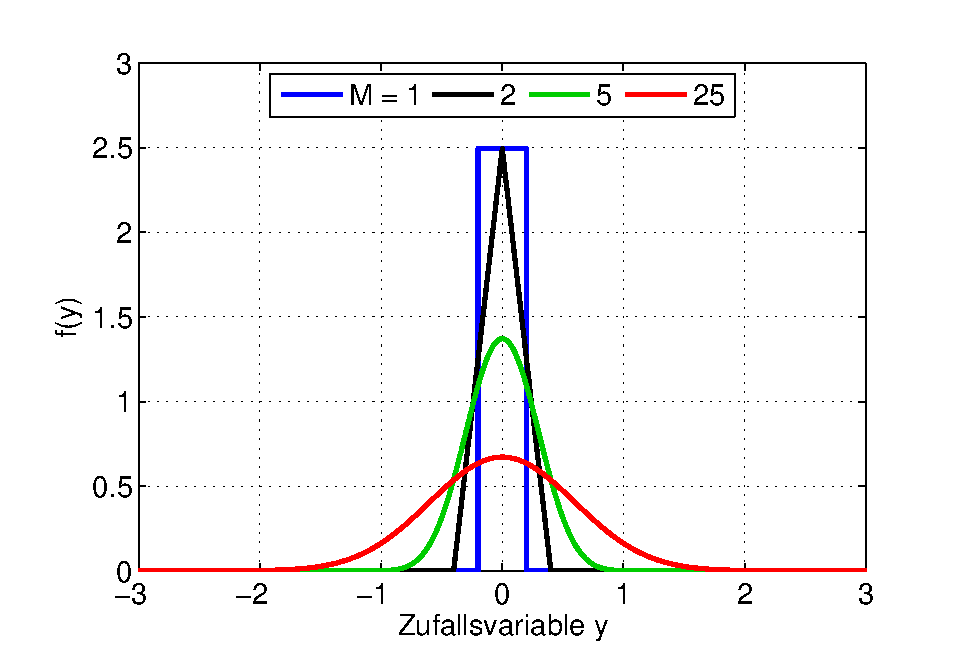
\includegraphics[width=0.5\textwidth]{Kapitel8/Bilder/image6}}
  \caption{Wahrscheinlichkeitsdichte der Zufallsvariablen y bei unterschiedlicher Anzahl summierter Zufallsvariablen}
  \label{fig:Grenzwertsatz1}
\end{figure}

\noindent Die Wahrscheinlichkeitsdichte f(y) wird mit steigendem m breiter und n\"{a}hert sich in ihrer Form der Standardnormalverteilung zunehmend an. In Bild \ref{fig:Grenzwertsatz2} wird f\"{u}r M = 25 die Verteilung der Zufallsvariable 

\begin{equation}\label{eq:eightsixtyseven}
z=\dfrac{y-M\cdot \mu}{\sigma \cdot \sqrt{M}}
\end{equation}

\noindent mit einer Standardnormalverteilung verglichen.

\noindent 
\begin{figure}[H]
  \centerline{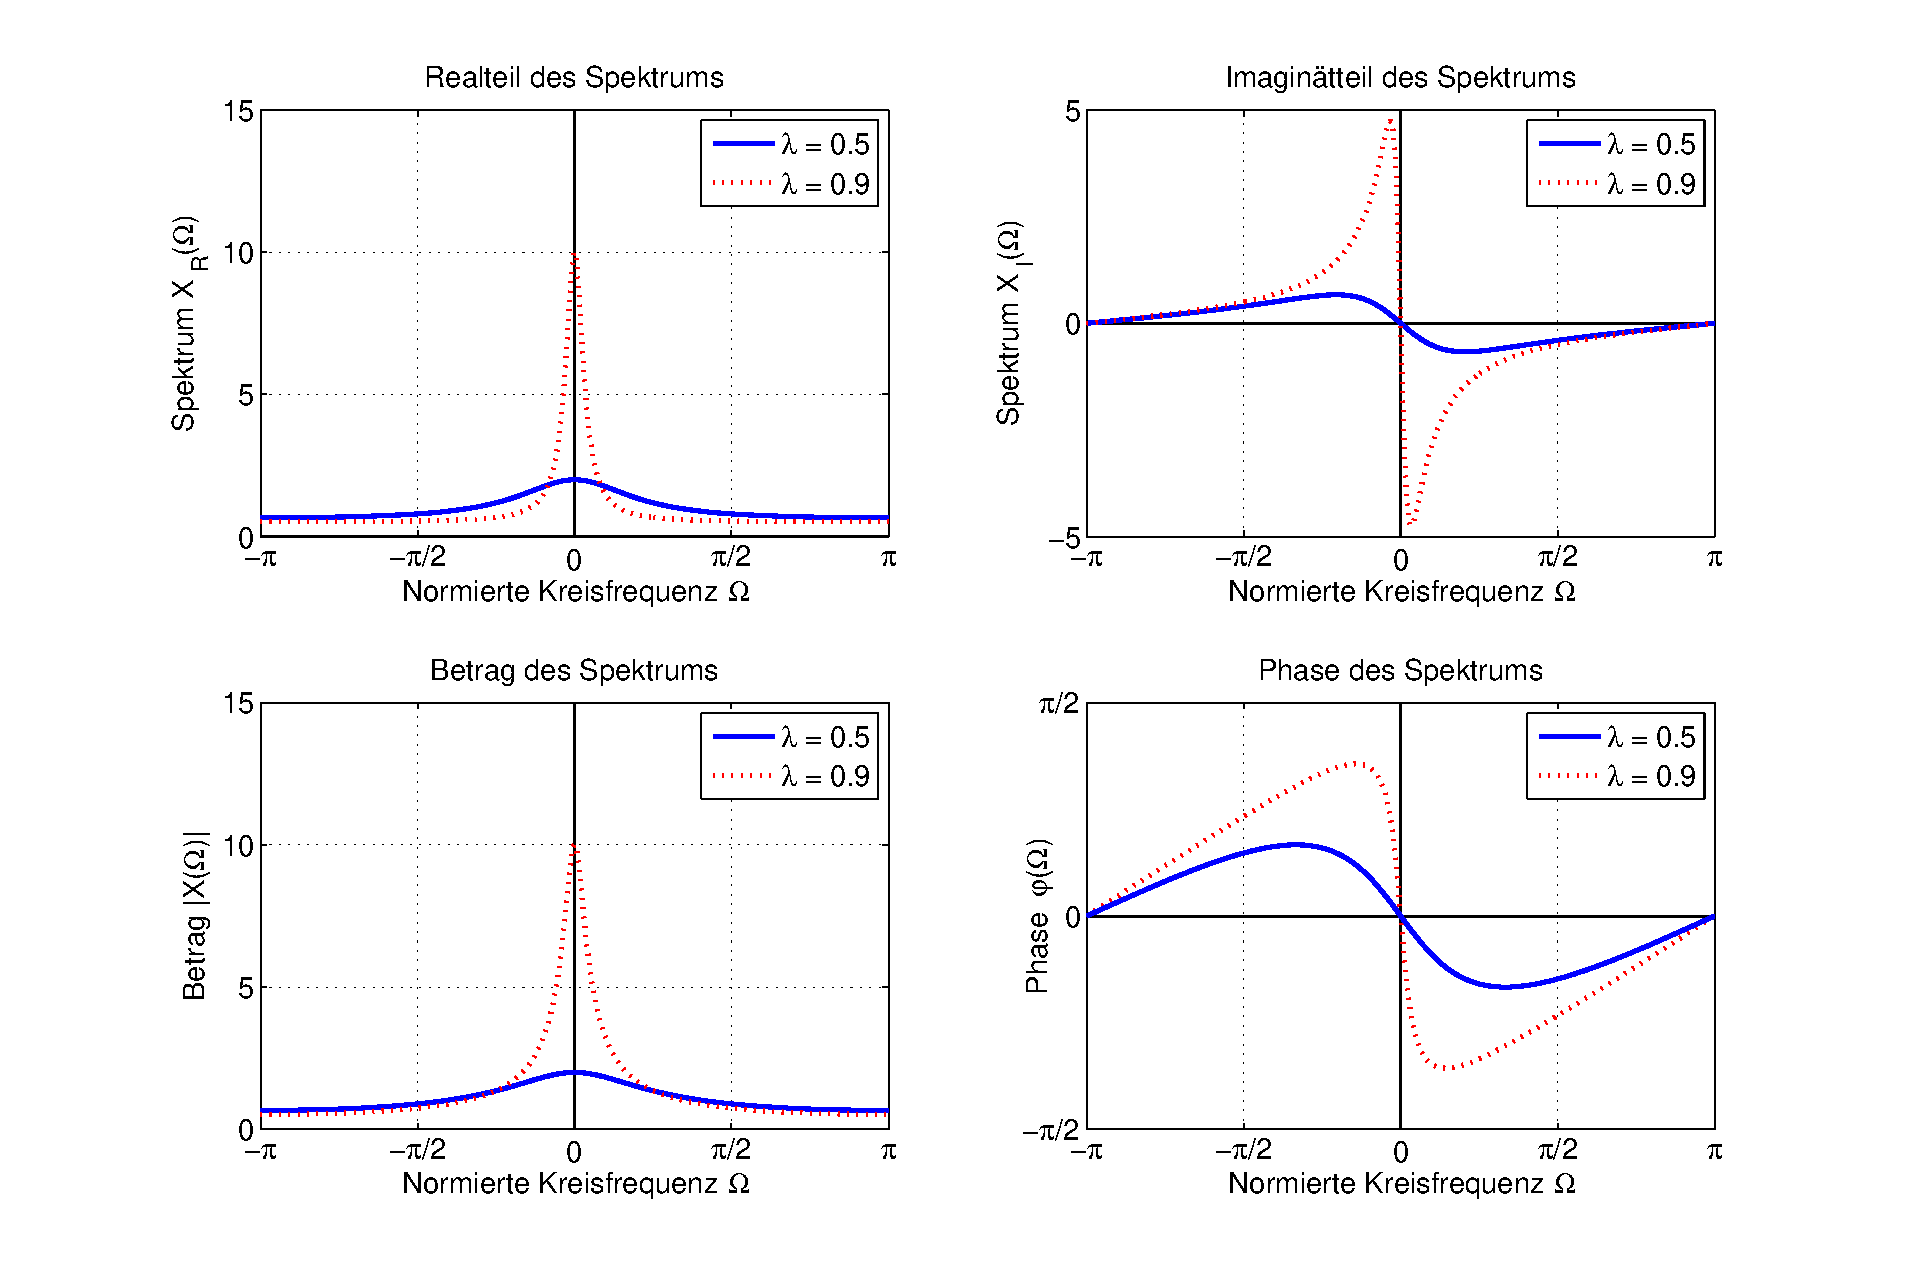
\includegraphics[width=0.5\textwidth]{Kapitel8/Bilder/image7}}
  \caption{Wahrscheinlichkeitsdichte der Zufallsvariabel z im Vergleich zur Standardnormalverteilung}
  \label{fig:Grenzwertsatz2}
\end{figure}

\noindent Es zeigt sich eine gute grafische \"{U}bereinstimmung der beiden Wahrscheinlichkeitsdichten, sodass das Beispiel den zentralen Grenzwertsatz grafisch best\"{a}tigt. Die G\"{u}te der \"{U}bereinstimmung ist von der Anzahl der Stichproben M abh\"{a}ngig. Wie gro{\ss} die Anzahl erforderlicher Stichproben M ist, um eine ausreichend gute N\"{a}herung der Standardnormalverteilung zu erhalten, kann nicht pauschal beantwortet werden. Die Anzahl notwendiger Stichproben ist von der Wahrscheinlichkeitsdichte $f_{xm}(x_{m})$ der Zufallsvariablen $x_{m}$ und der Aufgabenstellung abh\"{a}ngig. In dem Beispiel zeigt sich f\"{u}r M = 25 eine gute \"{U}bereinstimmung, in der Literatur wird der Wert M = 30 f\"{u}r eine gute Approximation angegeben. Oft reichen aber auch bereits erheblich weniger Stichproben aus, um mit der Normalverteilung n\"{a}herungsweise rechnen zu k\"{o}nnen.

\clearpage

\subsection{Spezielle multivariate Verteilungen}

\noindent Abschlie{\ss}end werden mit der Multinomial-Verteilung f\"{u}r diskrete Variablen und der multivariaten Normalverteilung f\"{u}r stetige Variablen die beiden wichtigsten multivariaten Verteilungen eingef\"{u}hrt.

\subsubsection{Multinomial-Verteilung}

\noindent Die Multinomial-Verteilung ergibt sich als Verallgemeinerung der Binomial-Verteilung. Wenn f\"{u}r einen Zufallsprozess M sich gegenseitig ausschlie{\ss}ende Ausg\"{a}nge m\"{o}glich sind und der Zufallsprozess N-mal unabh\"{a}ngig wiederholt wird, k\"{o}nnen die Wahrscheinlichkeiten mithilfe der Multinomial-Verteilung berechnet werden. Dabei hat jedes m\"{o}gliche Ereignis $x_{1}$, {\dots}, $x_{M}$ eine Auftretenswahrscheinlichkeit von $p_{1}$, {\dots}, $p_{M}$. Die Wahrscheinlichkeitsfunktion eines multinomialverteilten Zufallsvektors

\begin{equation}\label{eq:eightsixtyeight}
\underline{x}=(x_{1} ,...,x_{M})
\end{equation}

\noindent ist dabei definiert durch

\begin{equation}\label{eq:eightsixtynine}
\begin{split}
f\left(\underline{x}\right) & = f(x_{1} ,...,x_{M})=\dfrac{N!}{\prod _{m=1}^{M-1}x_{m} ! \cdot \left(N-\sum _{m=1}^{M-1}x_{m} \right)!} \cdot \prod _{m=1}^{M-1}p_{m}^{x_{m}} \cdot \left(1-\sum _{m=1}^{M-1}p_{m} \right)^{N-\sum _{m=1}^{M-1}x_{m}}
\end{split}
\end{equation}

\noindent Die durch Gleichung \eqref{eq:eightsixtynine} definierte Multinomial-Verteilung f\"{u}r zwei Dimensionen mit p$_{1}$=1/2, p$_{2}$=1/3 und p$_{3}$=1/6 bei N = 10 Wiederholungen ist in Bild \ref{fig:MultinomialVerteilung1} zu sehen.

\noindent 
\begin{figure}[H]
  \centerline{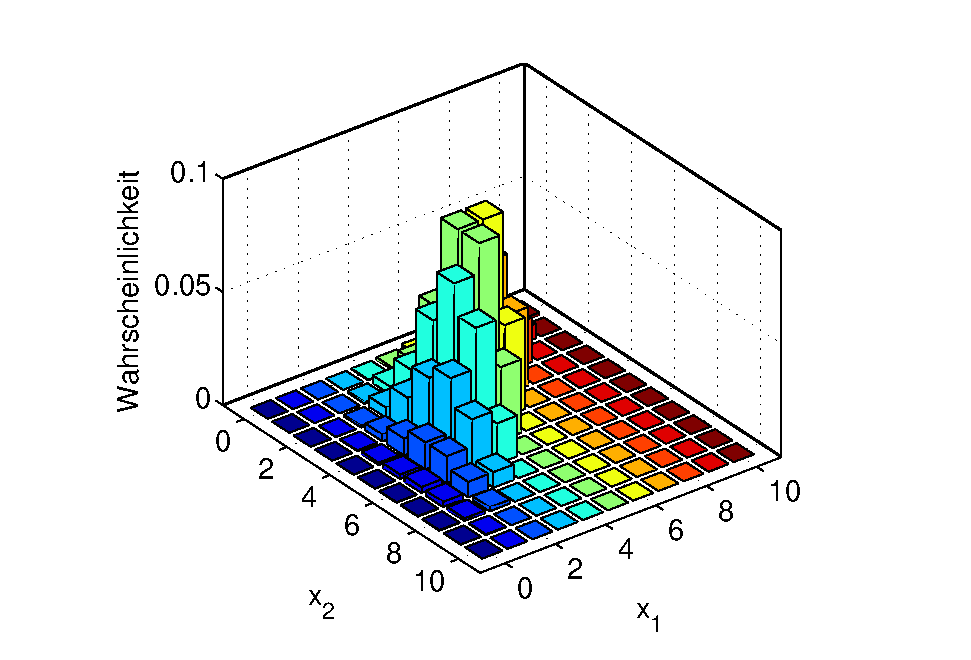
\includegraphics[width=0.5\textwidth]{Kapitel8/Bilder/image8}}
  \caption{Grafische Darstellung der zweidimensionalen Multinomial-Verteilung mitp$_{1}$=1/2, p$_{2}$=1/3 und p$_{3}$=1/6}
  \label{fig:MultinomialVerteilung1}
\end{figure}

\noindent F\"{u}r den Spezialfall von M = 2 f\"{u}hrt Gleichung \eqref{eq:eightsixtynine} zu der aus Kapitel 4 bekannten Binomial-Verteilung, die durch die Gleichung

\begin{equation}\label{eq:eightseventy}
f(x_{1})=\dfrac{N!}{x_{1} \cdot (N-x_{1} )!} \cdot p_{1}^{x_{1} } \cdot (1-p_{1})^{N-x_{1} }
\end{equation}

\noindent beschrieben ist. Die Wahrscheinlichkeit f\"{u}r eine durch den Vektor \underbar{x} gekennzeichnete Wertekombination berechnet sich durch

\begin{equation}\label{eq:eightseventyone}
P(\underline{x})=P(x_{1} ,...,x_{M})=\dfrac{N!}{\prod _{m=1}^{M}x_{m} !} \cdot \prod _{m=1}^{M}p_{m}^{x_{m} }
\end{equation}

\noindent Das Zufallsexperiment wird N-mal ausgef\"{u}hrt. Damit ist die Wahrscheinlichkeit f\"{u}r eine Anzahl von Ereignissen

\begin{equation}\label{eq:eightseventytwo}
P\left(\sum _{m=1}^{M}x_{m}  \ne N\right)=0
\end{equation}

\noindent Die Verteilungsfunktion der Multinomial-Verteilung ergibt sich durch Summation \"{u}ber die Wahrscheinlichkeitsfunktion zu

\begin{equation}\label{eq:eightseventythree}
P\left(\underline{\xi }\le \underline{x}\right)=F\left(\underline{x}\right)=F\left(x_{1} ,...,x_{M} \right)=\sum _{\xi _{M} =1}^{x_{M} }... \sum _{\xi _{1} =1}^{x_{1} }f\left(\xi _{1} ,...,\xi _{M} \right)
\end{equation}

\noindent Die Randverteilungen der Multinomial-Verteilung entsprechen den Binomialverteilungen der entsprechenden Variablen. Die Anwendung der Multinomial-Verteilung soll anhand eines Beispiels verdeutlicht werden.\bigskip

\noindent
\colorbox{lightgray}{%
\arrayrulecolor{white}%
\renewcommand\arraystretch{0.6}%
\begin{tabular}{ wl{16.5cm} }
{\fontfamily{phv}\selectfont
\noindent{Beispiel: Schaltschrankfertigung}}
\end{tabular}%
}\medskip

\noindent Als Beispiel f\"{u}r eine Multinomial-Verteilung wird eine Schaltschrankfertigung betrachtet. In einer Woche werden an vier Montagepl\"{a}tzen jeweils ein Schaltschrank hergestellt und gepr\"{u}ft. Es ist bekannt, dass die Schaltschr\"{a}nke mit einer Wahrscheinlichkeit von $p_{1} = 0.85$ vollst\"{a}ndig funktionst\"{u}chtig sind, mit einer Wahrscheinlichkeit von $p_{2} = 0.1$ w\"{a}hrend der Pr\"{u}fung geringf\"{u}gig nachgearbeitet werden m\"{u}ssen und mit einer Wahrscheinlichkeit von $p_{3} = 0.05$ in der folgenden Woche nachgearbeitet werden m\"{u}ssen und nicht termingerecht ausgeliefert werden k\"{o}nnen.\newline

\noindent Im Folgenden wird die Verteilung der Schaltschrankqualit\"{a}t beschrieben. Die Zufallsvariable $x_{1}$ beschreibt die Anzahl vollst\"{a}ndig funktionst\"{u}chtiger Schaltschr\"{a}nke, die Zufallsvariable $x_{2}$ die Anzahl der geringf\"{u}gig nachzuarbeitenden Schaltschr\"{a}nke und die Zufallsvariable $x_{3}$ die Anzahl der nicht termingerecht auslieferbaren Schaltschr\"{a}nke.\newline 

\noindent Die Gleichung zur Bestimmung der Wahrscheinlichkeiten f\"{u}r die einzelnen m\"{o}glichen Ausg\"{a}nge des Zufallsexperimentes lassen sich mit Gleichung \eqref{eq:eightseventyone} mit der Nebenbedingung

\begin{equation}\label{eq:eightseventyfour}
\sum _{m=1}^{M}x_{m} =N
\end{equation}

\noindent berechnen. Die Wahrscheinlichkeit f\"{u}r eine bestimmte Kombination errechnet sich zu

\begin{equation}\label{eq:eightseventyfive}
\begin{split}
P(x_{1} ,x_{2} ,x_{3}) & = \dfrac{N!}{x_{1} !\cdot x_{2} !\cdot x_{3} !} \cdot p^{x_{1}} \cdot p^{x_{2}} \cdot p^{x_{3}}\\
& = \dfrac{N!}{x_{1} !\cdot x_{2} !\cdot (4-(x_{1}+x_{2}))!} \cdot 0.85^{x_{1}} \cdot 0.1^{x_{2}} \cdot 0.05^{4-(x_{1}-x_{2})}
\end{split}
\end{equation}

\clearpage

\noindent Mit den Zufallsgr\"{o}{\ss}en $x_{1}$, $x_{2}$ und der Beziehung $x_{3} = N - x_{1} - x_{2}$ ist es ausreichend, zwei der drei m\"{o}glichen Ergebnisse der Zufallsexperimente anzugeben. Die dritte Zufallsvariable ist linear abh\"{a}ngig. Die Wahrscheinlichkeiten nach Gleichung \eqref{eq:eightseventyfive} sind in Tabelle \ref{tab:eightfive} zusammengefasst. Zus\"{a}tzlich zu den Auftretenswahrscheinlichkeiten sind in Tabelle 8.5 noch die Zeilen- und Spaltensummen eingetragen, die den Randverteilungen der Zufallsvariablen $x_{1}$ und $x_{2}$ entsprechen. Diese gen\"{u}gen der Binomialverteilung, die bereits aus Kapitel \ref{four} bekannt ist.

\begin{table}[H]
\setlength{\arrayrulewidth}{.1em}
\caption{Wahrscheinlichkeiten des Zufallsexperimentes Schaltschrankbau}
\setlength{\fboxsep}{0pt}%
\colorbox{lightgray}{%
\arrayrulecolor{white}%
\begin{tabular}{| wc{1.75cm}  wc{1.65cm} | wc{1.7cm} | wc{1.7cm} | wc{1.7cm} | wc{1.7cm} | wc{1.7cm} | wc{1.7cm} }
\xrowht{10pt}

& & 
\multicolumn{5}{c|}{\fontfamily{phv}\selectfont\textbf{Zufallsvariable x$_{2}$}} &
\multirow{2}{*}{\fontfamily{phv}\selectfont\textbf{f$_{x_{1}}$(x$_{x_{1}}$)}}\\  \xrowht{10pt} 

& & 
\fontfamily{phv}\selectfont\textbf{0} &
\fontfamily{phv}\selectfont\textbf{1} &
\fontfamily{phv}\selectfont\textbf{2} &
\fontfamily{phv}\selectfont\textbf{3} &
\fontfamily{phv}\selectfont\textbf{4}  \\ \hline \xrowht{10pt} 

\multirow{5.5}{*}{\fontfamily{phv}\selectfont\textbf{Zufalls-}}& 
\fontfamily{phv}\selectfont\textbf{0} & 
\fontfamily{phv}\selectfont{0.000} &
\fontfamily{phv}\selectfont{0.000} &
\fontfamily{phv}\selectfont{0.000} &
\fontfamily{phv}\selectfont{0.000} &
\fontfamily{phv}\selectfont{0.000} & 
\fontfamily{phv}\selectfont{0.000}\\ \cline{2-8} \xrowht{10pt} 

\multirow{5.8}{*}{\fontfamily{phv}\selectfont\textbf{variable}} & 
\fontfamily{phv}\selectfont\textbf{1} & 
\fontfamily{phv}\selectfont{0.000} &
\fontfamily{phv}\selectfont{0.003} &
\fontfamily{phv}\selectfont{0.005} &
\fontfamily{phv}\selectfont{0.003} &
\fontfamily{phv}\selectfont{0} & 
\fontfamily{phv}\selectfont{0.011}\\ \cline{2-8} \xrowht{10pt} 

\multirow{6.1}{*}{\fontfamily{phv}\selectfont\textbf{$x_{1}$}}& 
\fontfamily{phv}\selectfont\textbf{2} & 
\fontfamily{phv}\selectfont{0.011} &
\fontfamily{phv}\selectfont{0.043} &
\fontfamily{phv}\selectfont{0.043} &
\fontfamily{phv}\selectfont{0} &
\fontfamily{phv}\selectfont{0} & 
\fontfamily{phv}\selectfont{0.097}\\ \cline{2-8} \xrowht{10pt} 

& 
\fontfamily{phv}\selectfont\textbf{3} & 
\fontfamily{phv}\selectfont{0.123} &
\fontfamily{phv}\selectfont{0.246} &
\fontfamily{phv}\selectfont{0} &
\fontfamily{phv}\selectfont{0} &
\fontfamily{phv}\selectfont{0} & 
\fontfamily{phv}\selectfont{0.369}\\ \cline{2-8} \xrowht{10pt} 

& 
\fontfamily{phv}\selectfont\textbf{4} & 
\fontfamily{phv}\selectfont{0.522} &
\fontfamily{phv}\selectfont{0} &
\fontfamily{phv}\selectfont{0} &
\fontfamily{phv}\selectfont{0} &
\fontfamily{phv}\selectfont{0} & 
\fontfamily{phv}\selectfont{0.522}\\ \hline \xrowht{10pt} 

\fontfamily{phv}\selectfont\textbf{f$_{x_{2}}$(x$_{2}$)} &
&
\fontfamily{phv}\selectfont{0.656} &
\fontfamily{phv}\selectfont{0.292} &
\fontfamily{phv}\selectfont{0.048} &
\fontfamily{phv}\selectfont{0.003} &
\fontfamily{phv}\selectfont{0.000} &
\fontfamily{phv}\selectfont{1}\\ \hline

\end{tabular}%
}\bigskip
\label{tab:eightfive}
\end{table}

\noindent Die Wahrscheinlichkeiten f\"{u}r das Eintreten einer bestimmten Anzahl $x_{1}$ von vollst\"{a}ndig funktionsf\"{a}higen und einer bestimmten Anzahl $x_{2}$ von geringf\"{u}gig nachzuarbeitenden Schaltschr\"{a}nken lassen sich grafisch darstellen. Dies ist in Bild \ref{fig:MultinomialVerteilung2} zu sehen.

\noindent 
\begin{figure}[H]
  \centerline{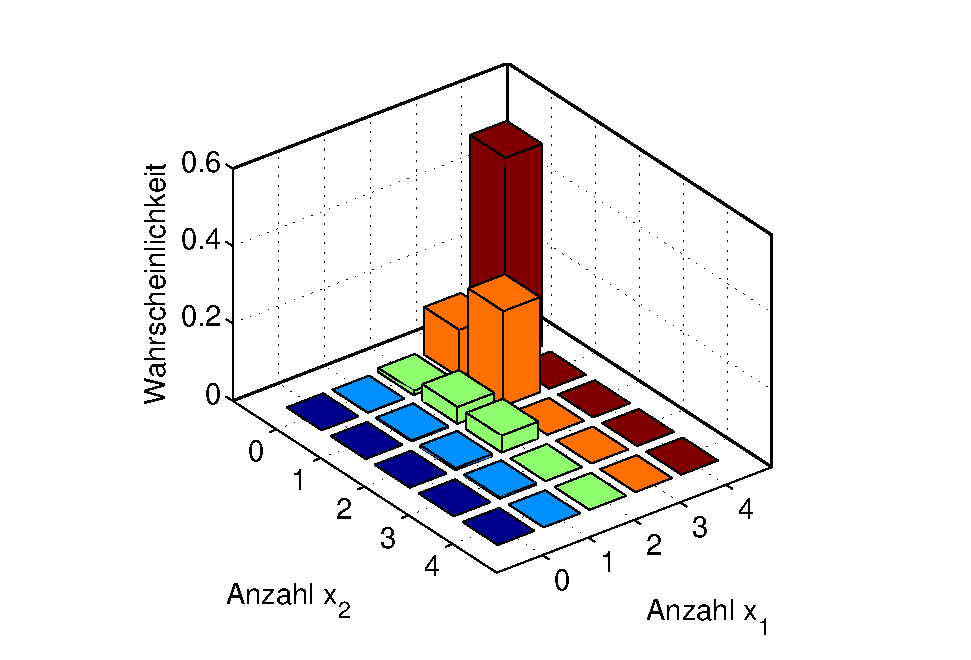
\includegraphics[width=0.5\textwidth]{Kapitel8/Bilder/image9}}
  \caption{Grafische Darstellung der Wahrscheinlichkeiten aus Tabelle \ref{tab:eightfive}}
  \label{fig:MultinomialVerteilung2}
\end{figure}

\noindent Die Wahrscheinlichkeit, dass alle Schaltschr\"{a}nke termingerecht ausgeliefert werden k\"{o}nnen, ergibt sich aus den F\"{a}llen, in denen die Summe der beiden Zufallsvariablen $x_{1}$ und $x_{2}$ bereits 4 ergibt. Nach Tabelle \ref{tab:eightfive} ergibt sich die Wahrscheinlichkeit 

\begin{equation}\label{eq:eightseventysix}
P(x_{3} =0)=0+0.003+0.043+0.246+0.522= 0.8140
\end{equation}

\clearpage

\noindent Die Berechnung erfolgte dabei mit MATLAB durch den folgenden Programmabschnitt.

\lstinputlisting[caption = {}]{Kapitel8/mat1.m}

\noindent In Python ergibt sich analog der folgende Programmausschnitt.

\lstinputlisting[caption = {}]{Kapitel8/mat2.m}

\subsubsection{Multivariate Normalverteilung}

\noindent Bei der multivariaten Normalverteilung handelt es sich um die Verallgemeinerung der eindimensionalen Normalverteilung. Sie tritt als Grenzwert von Summen unabh\"{a}ngiger mehrdimensionaler Zufallsvariablen auf. Dadurch kann die multivariate Normalverteilung dort angewandt werden, wo mehrdimensionale zuf\"{a}llige Gr\"{o}{\ss}en als \"{U}berlagerung von vielen voneinander unabh\"{a}ngigen Einzeleffekten angesehen werden k\"{o}nnen.\newline

\noindent Die univariate Normalverteilung wird in Kapitel \ref{four} beschrieben durch die Gleichung

\begin{equation}\label{eq:eightseventyseven}
f(x)=\dfrac{1}{\sigma \cdot \sqrt{2\cdot \pi}} \cdot e^{-\dfrac{1}{2} \cdot \left(\dfrac{x-\mu}{\sigma} \right)^{2}}
\end{equation}

\noindent Die multivariate Normalverteilung wird durch die beiden Verteilungsparameter \underbar{$\mu$} und \textbf{$\Sigma$} definiert, die den Parametern µ und $\sigma$ der univariaten Normalverteilung entsprechen. Eine Verallgemeinerung der in Gleichung \eqref{eq:eightseventyseven} angegebene univariate Normalverteilung f\"{u}r M-dimensionale Stichproben der Form

\begin{equation}\label{eq:eightseventyeight}
\underline{x}^{T} =\left(\begin{array}{ccc} {x_{1} } & {\cdots } & {x_{M} } \end{array}\right)
\end{equation}

\noindent f\"{u}hrt mit dem Mittelwertsvektor \underbar{$\mu$} und der Kovarianzmatrix \textbf{$\Sigma$} zu der Dichtefunktion der multivariaten Normalverteilung

\begin{equation}\label{eq:eightseventynine}
f\left(\underline{x}\right)=\dfrac{1}{\left|\Sigma \right|^{\dfrac{1}{2} } \cdot (2\cdot \pi)^{\dfrac{M}{2}}} \cdot e^{-\dfrac{1}{2} \cdot (X- M)^{T} \cdot (X- M)\cdot \Sigma ^{-1}}
\end{equation}

\noindent Wie bei der univariaten Normalverteilung liegt auf Grund der Symmetrie das Maximum der Verteilung an dem Punkt, der durch den Mittelwertsvektor \underbar{$\mu$} beschrieben ist. Bild \ref{fig:MultivarianteVerteilungen1} zeigt die Dichtefunktion einer zweidimensionalen Standardnormalverteilung der Zufallsvariablen x und y mit einem Mittelwertsvektor von

\begin{equation}\label{eq:eighteighty}
\underline{\mu }^{T} =\left(\begin{array}{cc} {\mu _{x} } & {\mu _{y} } \end{array}\right)=\left(\begin{array}{cc} {0} & {0} \end{array}\right)
\end{equation}

\noindent und einer Kovarianzmatrix von

\begin{equation}\label{eq:eighteightyone}
\Sigma =\left(\begin{array}{cc} {\sigma _{x}^{2} } & {\sigma _{xy}} \\ {\sigma _{xy}} & {\sigma _{y}^{2}} \end{array}\right)=\left(\begin{array}{cc} {1} & {0} \\ {0} & {1} \end{array}\right)
\end{equation}

\noindent 
\begin{figure}[H]
  \centerline{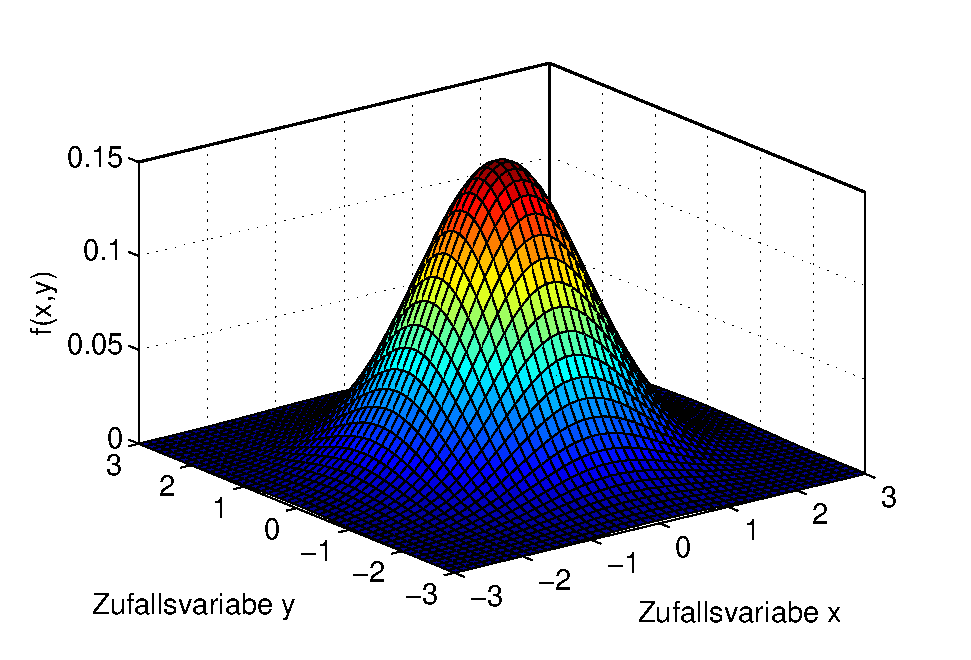
\includegraphics[width=0.5\textwidth]{Kapitel8/Bilder/image10}}
  \caption{R\"{a}umliche Darstellung der Dichtefunktion der multivariaten Standardnormalverteilung}
  \label{fig:MultivarianteVerteilungen1}
\end{figure}

\noindent Da es bei den r\"{a}umlichen Darstellungen nur schwer m\"{o}glich ist, den genauen Wert der Dichtefunktion f\"{u}r eine bestimmte Wertekonstellation abzulesen, wird stattdessen ein Kontur-Plot verwendet, der die Werte der Dichtefunktion auf eine Ebene projiziert. Bild \ref{fig:MultivarianteVerteilungen2} zeigt die multivariate Standardnormalverteilung als Kontur-Plot.

\noindent 
\begin{figure}[H]
  \centerline{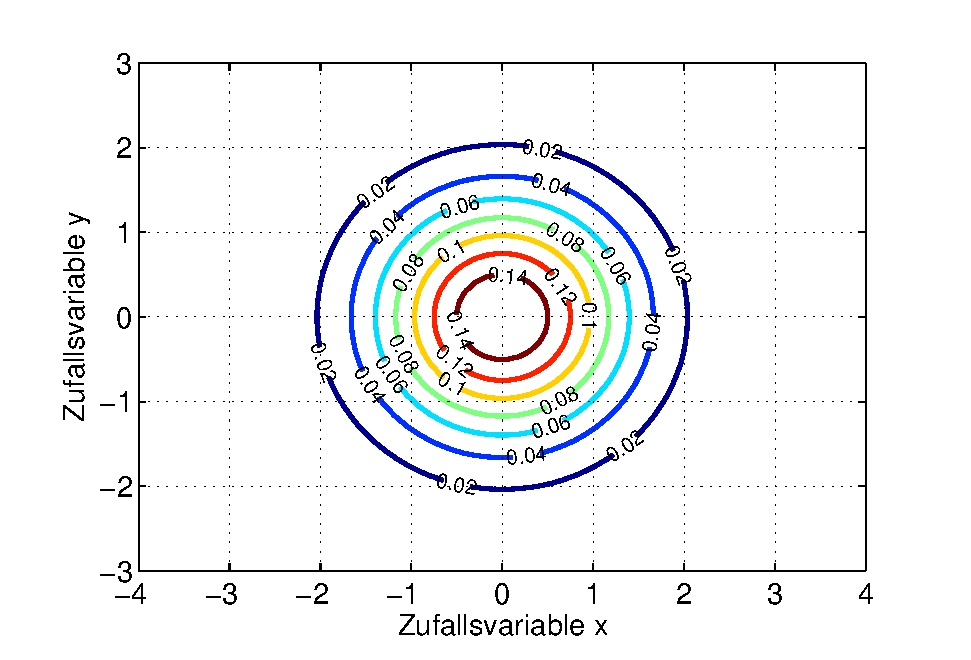
\includegraphics[width=0.5\textwidth]{Kapitel8/Bilder/image11}}
  \caption{Kontur-Plot der Dichtefunktion der multivariaten Standardnormalverteilung}
  \label{fig:MultivarianteVerteilungen2}
\end{figure}

\noindent Die Verteilungsfunktion der Standardnormalverteilung berechnet sich \"{u}ber die Integration zu

\begin{equation}\label{eq:eighteightytwo}
F(X)=\int\limits _{-\infty}^{X}\dfrac{1}{\left|\underline{\Sigma }\right|^{\dfrac{1}{2}} \cdot (2\cdot \pi)^{\dfrac{o}{2}}} \cdot e^{-\dfrac{1}{2} \cdot (\Xi - M)^{'} \cdot (\Xi-M)\cdot \underline{\Sigma}^{-1}} d\Xi
\end{equation}

\noindent Bild \ref{fig:MultivarianteVerteilungen3} zeigt Verteilungsfunktion der Standardnormalverteilung als r\"{a}umliche Darstellung und als Kontur-Plot.

\clearpage

\noindent 
\begin{figure}[H]
  \centerline{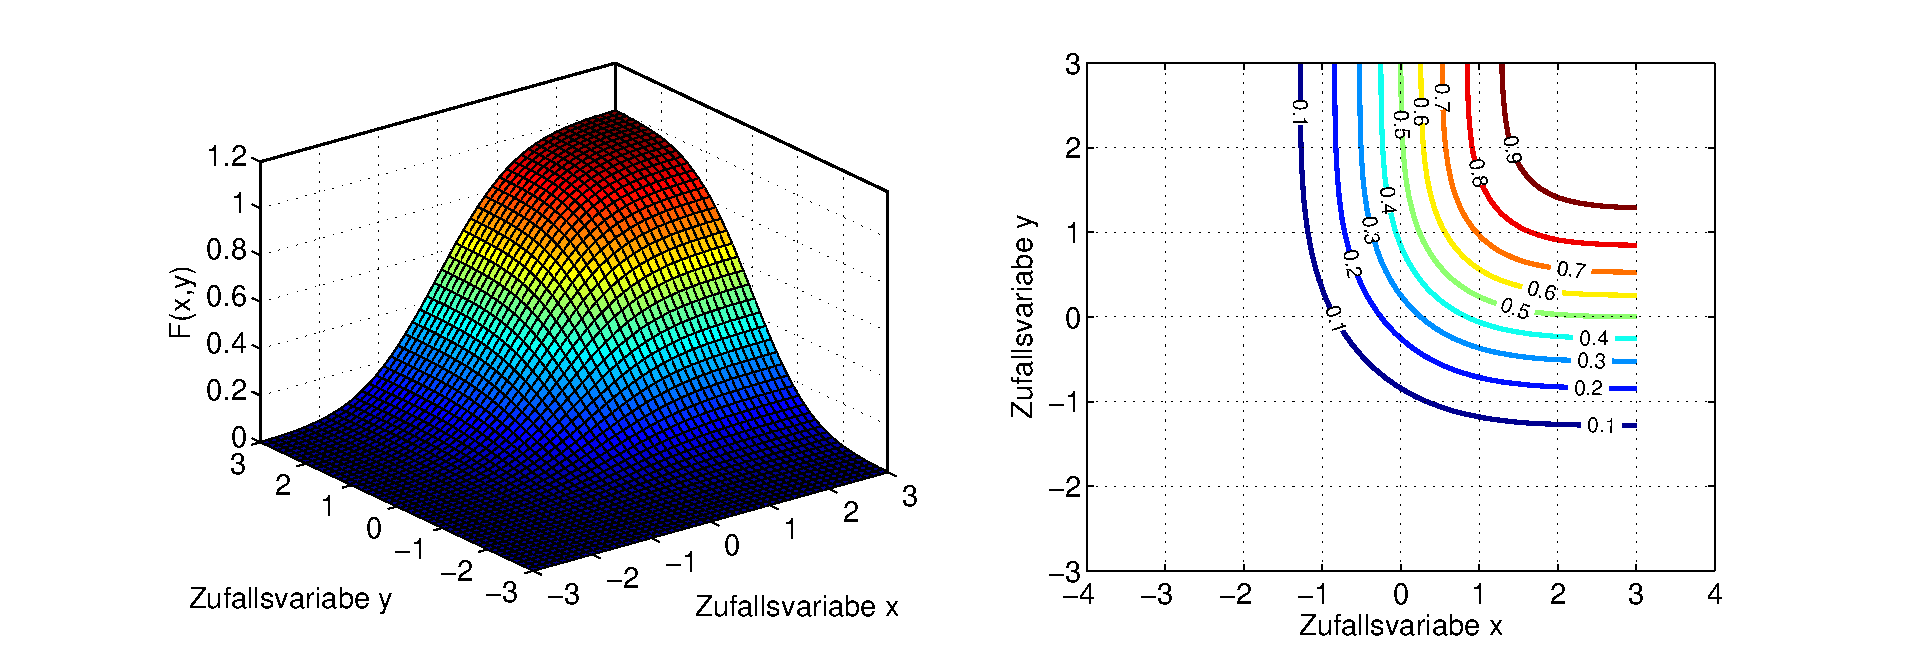
\includegraphics[width=1\textwidth]{Kapitel8/Bilder/image12}}
  \caption{Verteilungsfunktion der multivariaten Standardnormalverteilung}
  \label{fig:MultivarianteVerteilungen3}
\end{figure}

\noindent Die Randverteilungen der multivariaten Normalverteilung entsprechen der univariaten Normalverteilung, in diesem Fall der univariaten Standardnormalverteilung.\newline

\noindent F\"{u}r die multivariate Standardnormalverteilung sind die Zufallsgr\"{o}{\ss}en x und y unabh\"{a}ngig voneinander, da die Kovarianz der beiden Gr\"{o}{\ss}en den Wert 0 annimmt.

\begin{equation}\label{eq:eighteightythree}
\Sigma =\left(\begin{array}{cc} {\sigma _{x}^{2}} & {\sigma _{xy}} \\ {\sigma _{xy}} & {\sigma _{y}^{2}} \end{array}\right)=\left(\begin{array}{cc} {\sigma _{x}^{2}} & {0} \\ {0} & {\sigma _{y}^{2}} \end{array}\right)
\end{equation}

\noindent Sind die beiden Zufallsgr\"{o}{\ss}en wie bei der Standardnormalverteilung unabh\"{a}ngig voneinander, sind die Hauptachsen der Ellipse im Kontur-Plot parallel zu den beiden xy-Achsen ausgerichtet. Mit steigender Kovarianz ver\"{a}ndert sich der Winkel zwischen den Hauptachsen und den Diagrammachsen, er steigt mit wachsender Kovarianz von 0 $(\sigma_{xy} = 0)$ auf maximal $\pm 45\si{\degree} (\sigma_{xy} = \pm \infty)$ an. Die Randverteilungen bleiben dabei unver\"{a}ndert. Um dies zu verdeutlichen, wird in Bild \ref{fig:MultivarianteVerteilungen4} und Bild \ref{fig:MultivarianteVerteilungen5} die multivariate Normalverteilung mit unterschiedlichen Kovarianzmatrizen dargestellt. F\"{u}r die Darstellung in Bild \ref{fig:MultivarianteVerteilungen4} wurde eine zweidimensionale Normalverteilung mit einem Mittelwertsvektor von

\begin{equation}\label{eq:eighteightyfour}
\underline{\mu }^{T} =\left(\begin{array}{cc} {\mu _{x} } & {\mu _{y} } \end{array}\right)=\left(\begin{array}{cc} {0} & {0} \end{array}\right)
\end{equation}

\noindent und einer Kovarianzmatrix von

\begin{equation}\label{eq:eighteightyfive}
\Sigma =\left(\begin{array}{cc} {1} & {0.8} \\ {0.8} & {1} \end{array}\right)
\end{equation}

\noindent gew\"{a}hlt. Die beiden Zufallsvariablen besitzen demnach eine Kovarianz von $\sigma_{xy} = 0.8$. Zur Visualisierung werden sowohl die r\"{a}umliche Darstellung als auch der Kontur-Plot verwendet.

\clearpage

\noindent 
\begin{figure}[H]
  \centerline{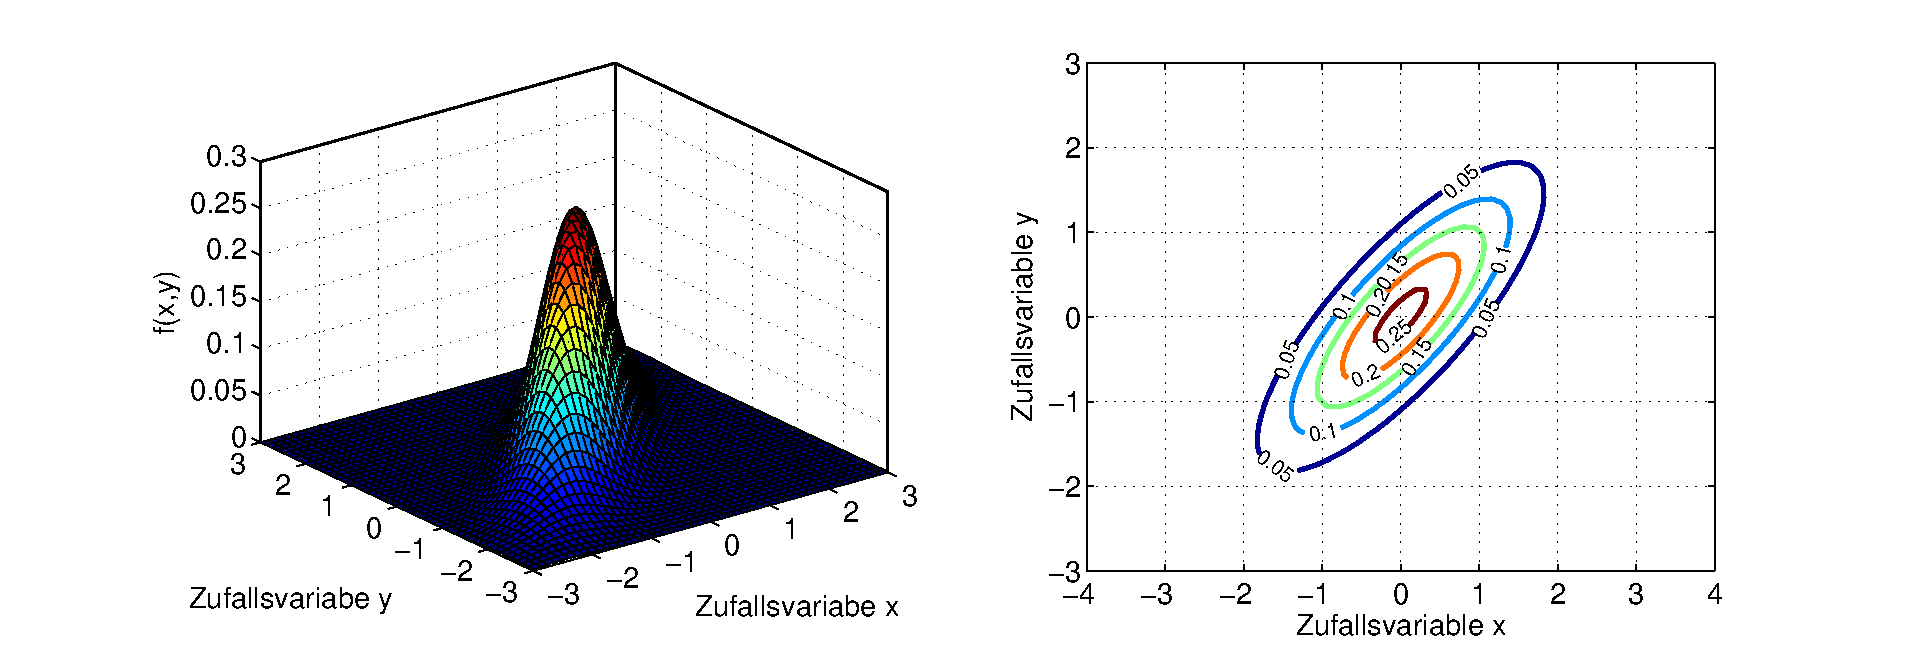
\includegraphics[width=1\textwidth]{Kapitel8/Bilder/image13}}
  \caption{ Dichtefunktion der multivariaten Standardnormalverteilung mit $\sigma_{xy} = 0.8$}
  \label{fig:MultivarianteVerteilungen4}
\end{figure}

\noindent Zum Vergleich zeigt Bild 8.14 die Dichtefunktion f\"{u}r eine Kovarianz von $\sigma_{xy} = -0.8$. 

\noindent 
\begin{figure}[H]
  \centerline{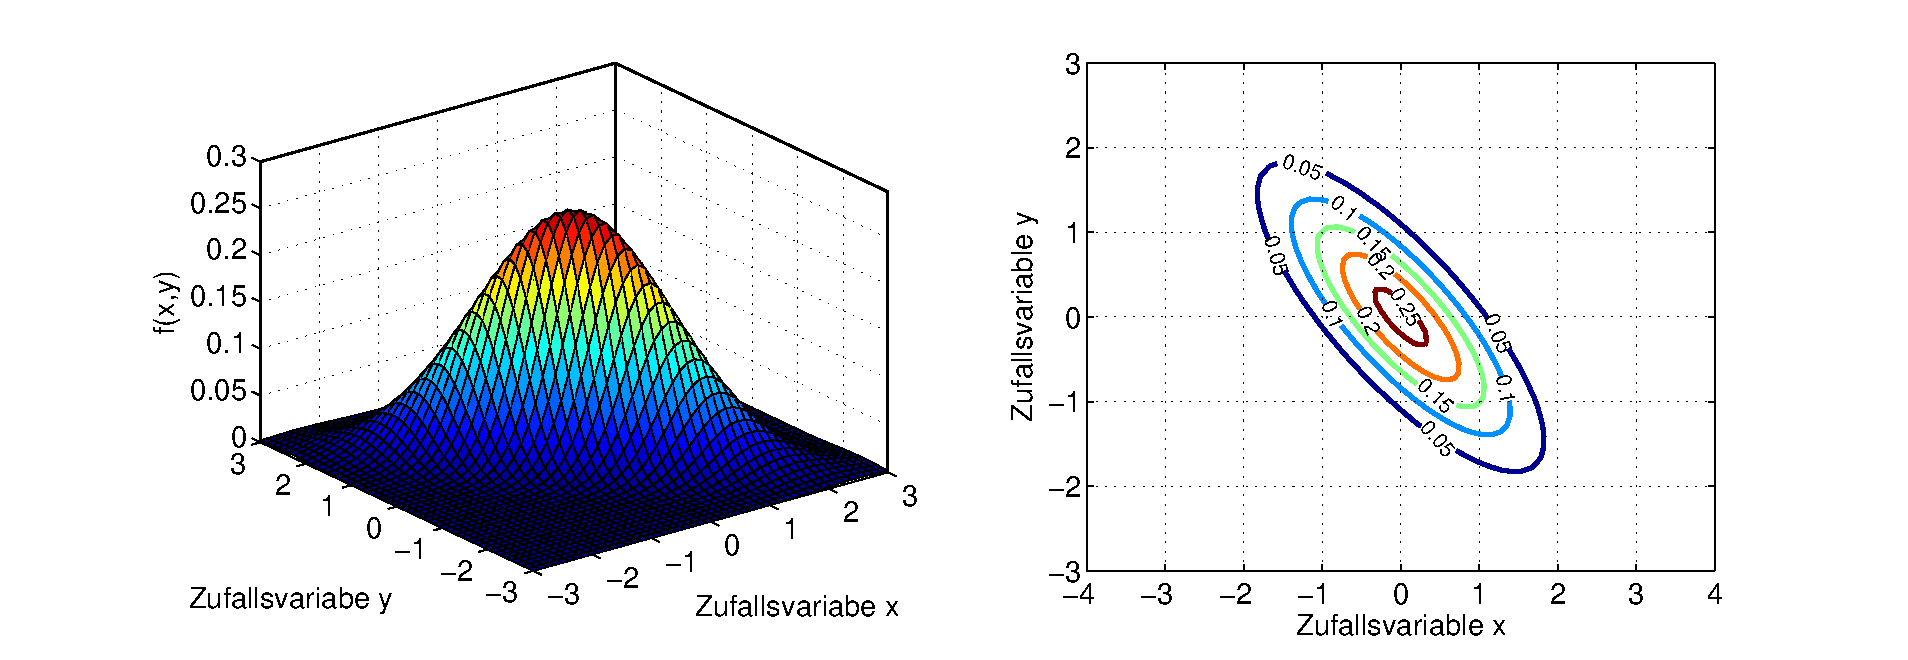
\includegraphics[width=1\textwidth]{Kapitel8/Bilder/image14}}
  \caption{ Dichtefunktion der multivariaten Standardnormalverteilung mit $\sigma_{xy} = -0.8$}
  \label{fig:MultivarianteVerteilungen5}
\end{figure}

\noindent Die Drehung der Dichtefunktion ist entgegengesetzt zu der vorigen Dichtefunktion in Bild \ref{fig:MultivarianteVerteilungen4}. Anhand der grafischen Darstellung kann abgelesen werden, ob die beteiligten Zufallsgr\"{o}{\ss}en abh\"{a}ngig voneinander sind und welches Vorzeichen die Kovarianz besitzt.\newline

\noindent In den bisherigen Beispielverteilungen in Bild \ref{fig:MultivarianteVerteilungen2}, Bild \ref{fig:MultivarianteVerteilungen4} oder Bild \ref{fig:MultivarianteVerteilungen5} waren die Zufallsgr\"{o}{\ss}en x und y stets standardnormalverteilt. In der Praxis ist dies ohne Zentrierung der Verteilung nur selten der Fall, meist liegt zus\"{a}tzlich eine Standardabweichung $\sigma$ ungleich 1 vor.\newline

\noindent In Bild \ref{fig:MultivarianteVerteilungen6} wird gezeigt, wie sich die multivariate Verteilungsfunktion \"{a}ndert, wenn die Verteilung der Zufallsvariable x durch eine Normalverteilung mit einem Mittelwert von $\mu_{x} = 0$ und einer Varianz von $\sigma_{xy} = 1.8$ beschrieben werden kann. Die Zufallsvariable y wird als standardnormalverteilt beibehalten. Beide Zufallsgr\"{o}{\ss}en sind voneinander unabh\"{a}ngig.

\clearpage

\noindent 
\begin{figure}[H]
  \centerline{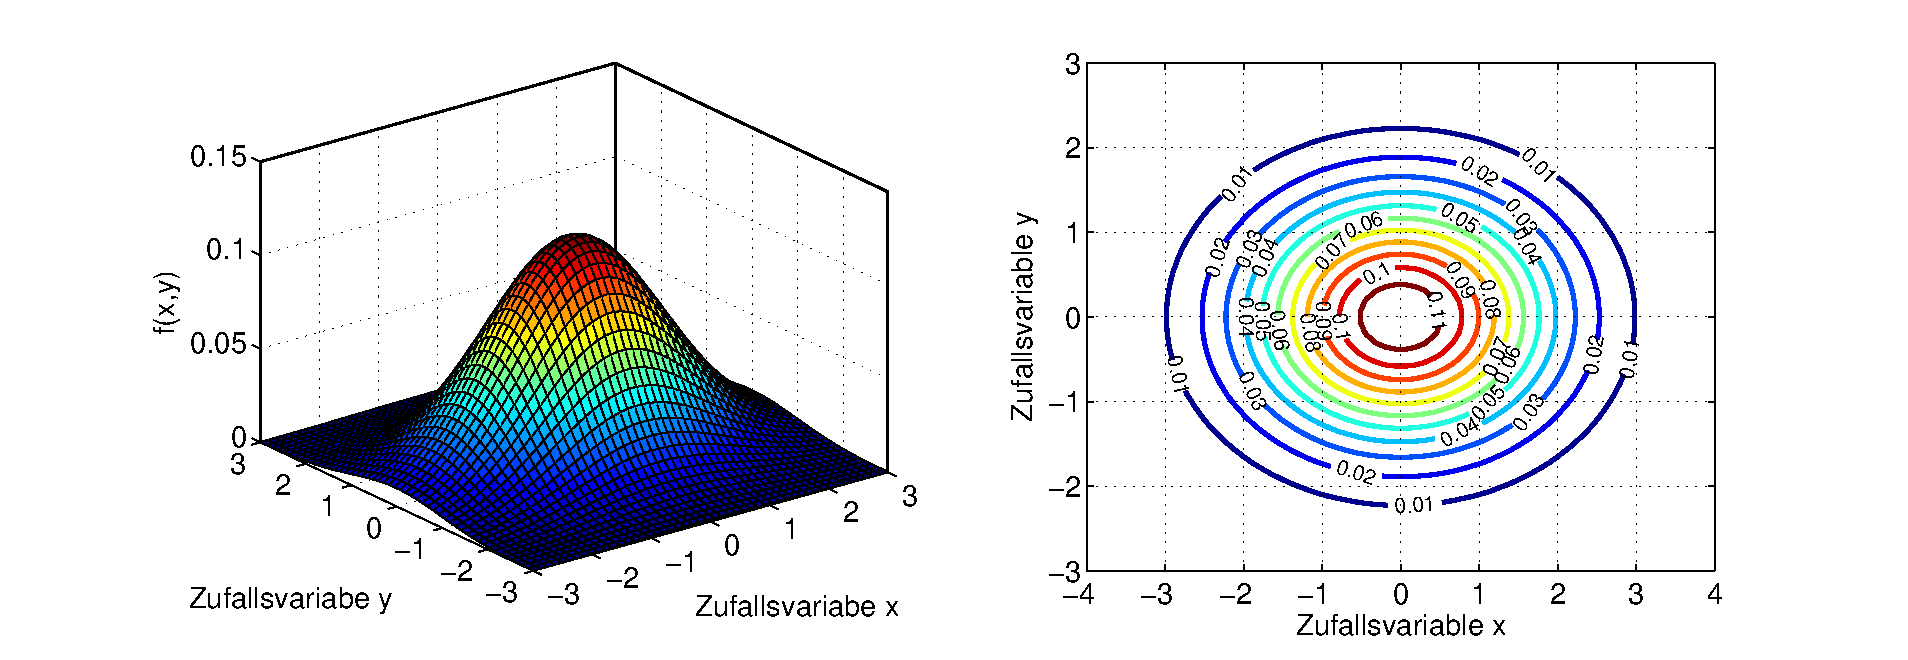
\includegraphics[width=1\textwidth]{Kapitel8/Bilder/image15}}
  \caption{ Dichtefunktion der multivariaten Standardnormalverteilung mit $\sigma_{x}^{2} = 1, \sigma_{y}^{2} = 0.5, \sigma_{xy} = 0$}
  \label{fig:MultivarianteVerteilungen6}
\end{figure}

\noindent Es ist zu erkennen, dass die Verteilung in Richtung der Zufallsvariablen x aufgrund der gr\"{o}{\ss}eren Streuung breiter geworden ist. 

\noindent Bild \ref{fig:MultivarianteVerteilungen7} zeigt die \"{A}nderung der multivariaten Verteilungsfunktion, wenn die Verteilung der Zufallsvariablen y mit einer Normalverteilung mit einem Mittelwert von $\mu_{y} = 0$ und einer Varianz von $\sigma_{y}^{2} = 0.5$ angenommen wird. Zur Veranschaulichung wird f\"{u}r die Darstellung die Verteilung der Zufallsvariablen x wieder als standardnormalverteilt angenommen. Beide Zufallsgr\"{o}{\ss}en sind voneinander unabh\"{a}ngig.

\noindent 
\begin{figure}[H]
  \centerline{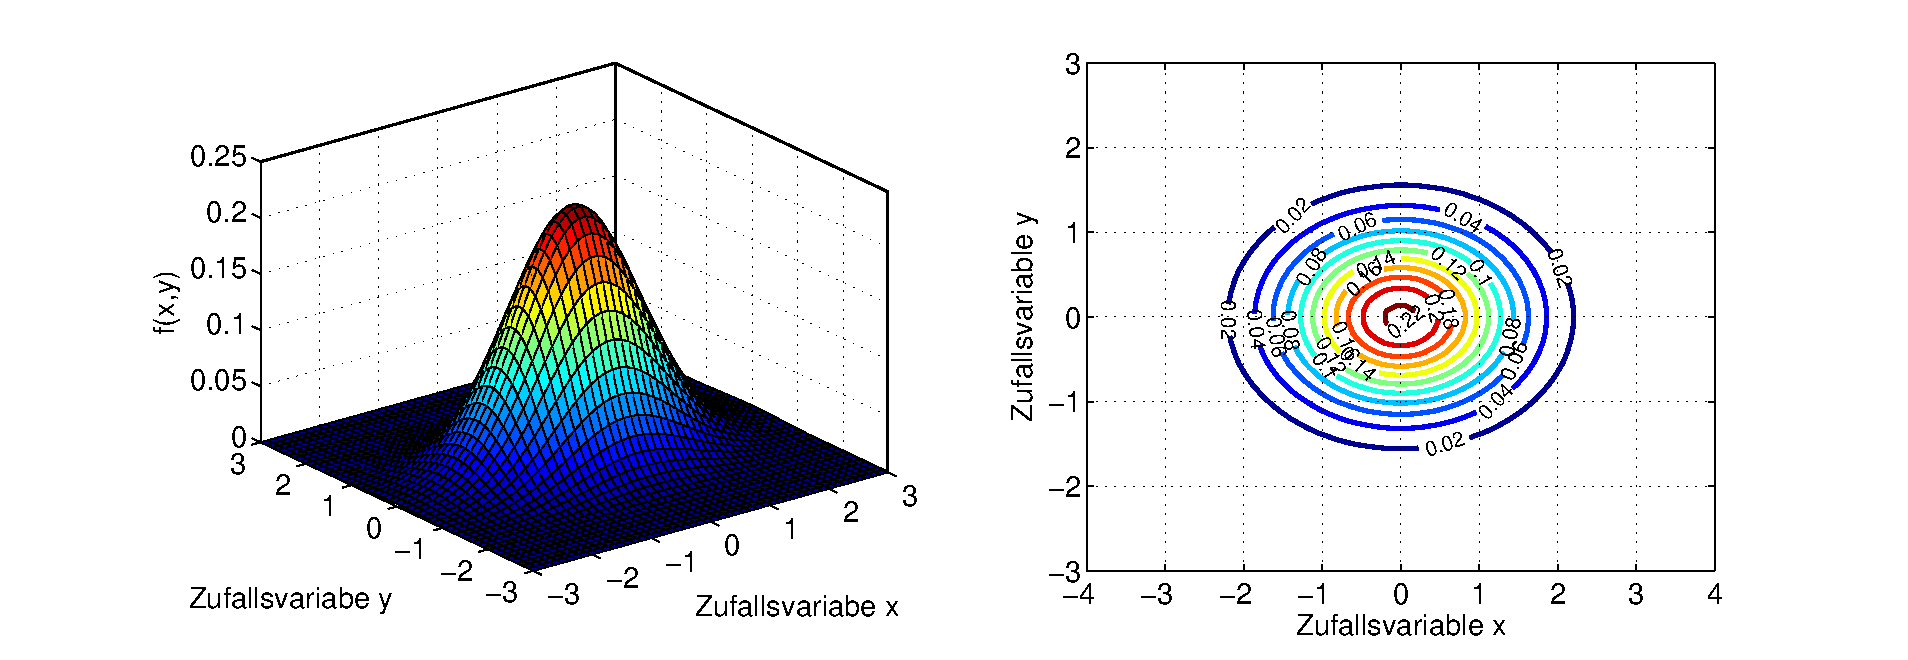
\includegraphics[width=1\textwidth]{Kapitel8/Bilder/image16}}
  \caption{ Dichtefunktion der multivariaten Standardnormalverteilung mit $\sigma_{x}^{2} = 1, \sigma_{y}^{2} = 0.5, \sigma_{xy} = 0$}
  \label{fig:MultivarianteVerteilungen7}
\end{figure}

\noindent In der Grafik ist gut zu erkennen, dass sich die Verteilung in Richtung der Zufallsvariablen y verschm\"{a}lert hat. Die multivariate Normalverteilung wird an einem Beispiel vertieft.\bigskip

\noindent
\colorbox{lightgray}{%
\arrayrulecolor{white}%
\renewcommand\arraystretch{0.6}%
\begin{tabular}{ wl{16.5cm} }
{\fontfamily{phv}\selectfont
\noindent{Beispiel: Qualit\"{a}tsbewertung von Temperaturwiderst\"{a}nden}}
\end{tabular}%
}\medskip

\noindent Als Beispiel f\"{u}r die multivariate Normalverteilung wird die Fertigung eines temperaturabh\"{a}ngigen Widerstandes untersucht. Er besitzt einen Widerstandswert von 

\begin{equation}\label{eq:eighteightysix}
R(T)=R_{20} \cdot \left(1+\alpha \cdot (T-T_{20} )\right)
\end{equation}

\noindent Es ist bekannt, dass der Widerstandswert R bei  $20 \si{\degree}C$ durch eine Normalverteilung mit einem Mittelwert von $\mu_{R} = 1000$ ? und einer Standardabweichung von $\sigma_{R}= 5$ ? beschrieben werden kann. Ebenso ist bekannt, dass auch der Temperaturkoeffizient $\alpha$ des Widerstandes durch eine Normalverteilung abgebildet werden kann. Der mittlere Wert des Temperaturkoeffizienten liegt bei $\mu = 3.85 10^{-3}/K$, die Standardabweichung betr\"{a}gt $\sigma_{C}=0.5 10^{-3}/K$. Die Kovarianz der beiden Gr\"{o}{\ss}en betr\"{a}gt $\sigma_{RC} = 1.63 m\Omega/K$. Mit den gegebenen Angaben ergibt sich der Mittelwertsvektor


\begin{equation}\label{eq:eighteightyseven}
\underline{\mu}^{T} =\left(\begin{array}{cc} {\mu _{R}} & {\mu _{C}} \end{array}\right)=\left(\begin{array}{cc} {1000 \Omega} & {3.85\cdot 10^{-3} /K} \end{array}\right)
\end{equation}

\noindent und die Kovarianzmatrix

\begin{equation}\label{eq:eighteightyeight}
\Sigma =\left(\begin{array}{cc} {\sigma _{R}^{2}} & {\sigma _{RC}} \\ {\sigma _{RC}} & {\sigma _{C}^{2}} \end{array}\right)=\left(\begin{array}{cc} {25 \Omega ^{2}} & {1.63 m\Omega /K} \\ {1.63 \Omega /K} & {0.25 10^{-6} /K^{2}} \end{array}\right)
\end{equation}

\noindent Durch die beiden Parameter \underbar{$\mu$} und \textbf{$\Sigma$} ist die multivariate Normalverteilung ausreichend spezifiziert. Die dazugeh\"{o}rige Dichteverteilung ist in Bild \ref{fig:Temperaturwiderstaende1} zu sehen.

\noindent 
\begin{figure}[H]
  \centerline{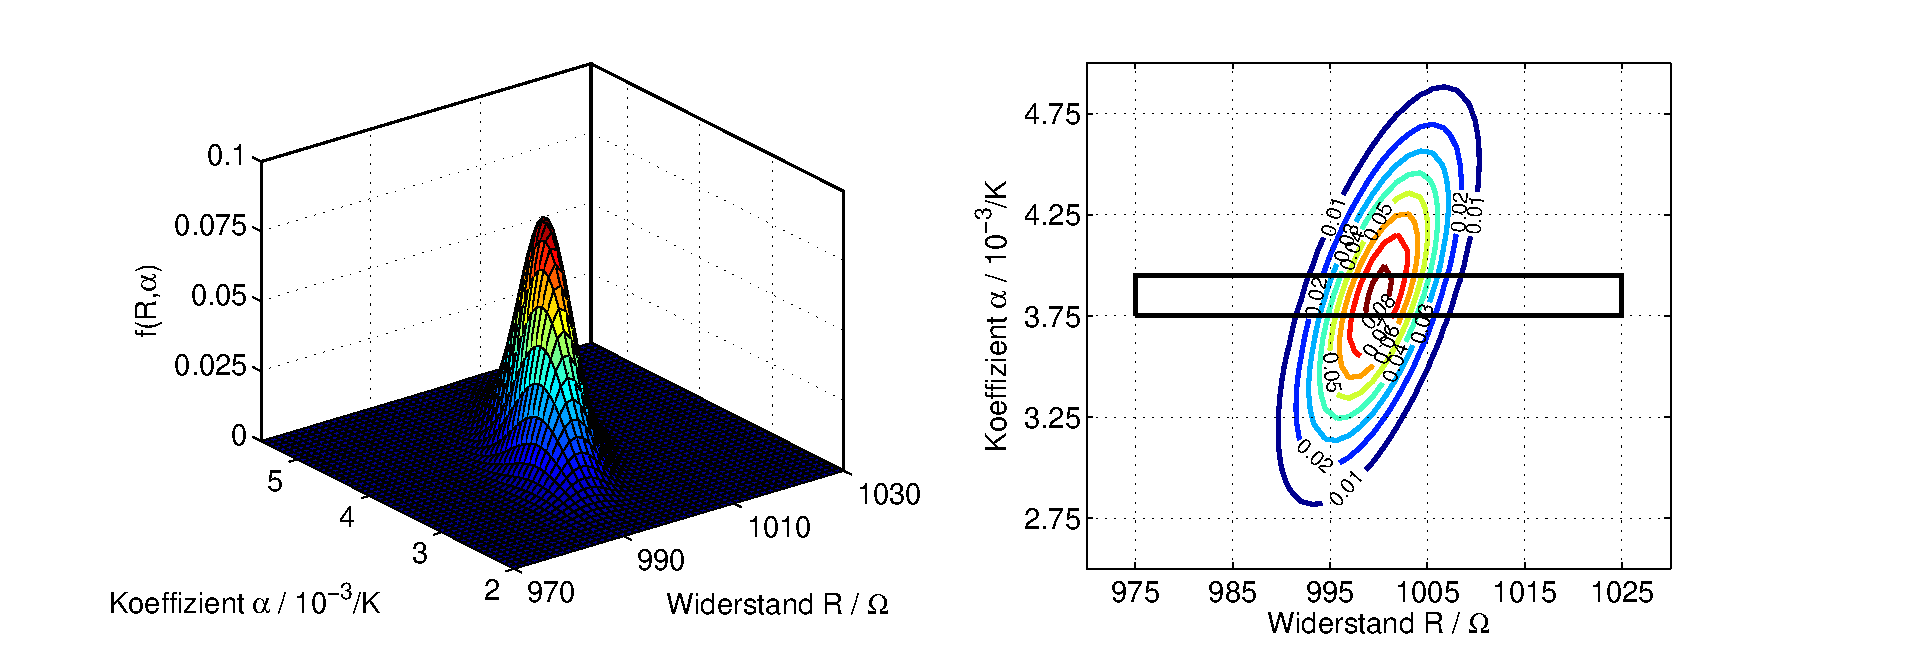
\includegraphics[width=1\textwidth]{Kapitel8/Bilder/image17}}
  \caption{Dichtefunktion der Temperaturwiderst\"{a}nde}
  \label{fig:Temperaturwiderstaende1}
\end{figure}

\noindent Bei der vorliegenden Widerstandsfertigung wird bewertet, wie viel Prozent der produzierten Temperaturwiderst\"{a}nde Ausschussware sind, wenn mit einem Kunden A eine Toleranz des Widerstandswertes und des Temperaturkoeffizienten von jeweils $\mathrm{\pm}$ 2.5 \% vereinbart wird. Der sich ergebende Bereich, in dem die Widerst\"{a}nde f\"{u}r Kunde A liegen d\"{u}rfen, ist exemplarisch in dem Kontur-Plot in Bild \ref{fig:Temperaturwiderstaende1} eingezeichnet. Mit einem Kunden B wird stattdessen eine erweiterte Toleranzgrenze von $\mathrm{\pm}$ 5 \% vereinbart. Die Berechnung erfolgt mithilfe der Verteilungsfunktion, die in Bild \ref{fig:Temperaturwiderstaende2} abgebildet ist. 

\noindent 
\begin{figure}[H]
  \centerline{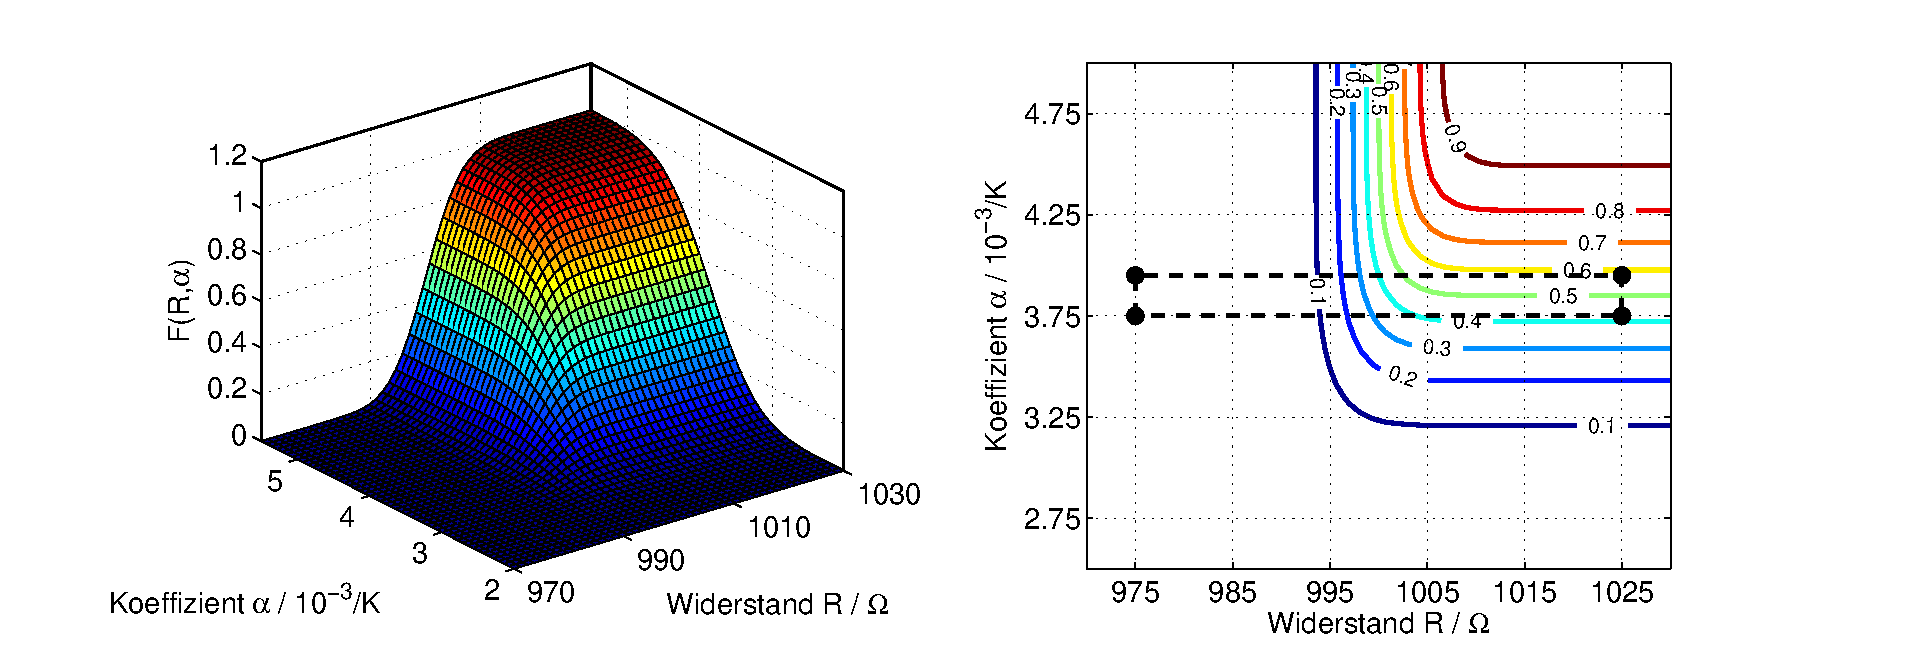
\includegraphics[width=1\textwidth]{Kapitel8/Bilder/image18}}
  \caption{Verteilungsfunktion der Temperaturwiderst\"{a}nde}
  \label{fig:Temperaturwiderstaende2}
\end{figure}

\noindent Die gesuchte Wahrscheinlichkeit f\"{u}r den Ausschussanteil bei Kunde A kann als die Fl\"{a}che au{\ss}erhalb des in Bild \ref{fig:Temperaturwiderstaende1} eingezeichneten Quadrates verstanden werden. Mithilfe der Verteilungsfunktion aus Bild \ref{fig:Temperaturwiderstaende2} kann die Wahrscheinlichkeit p f\"{u}r eine Fertigung innerhalb der Toleranzen berechnet werden zu 

\begin{equation}\label{eq:eighteightynine}
\begin{split}
p & =F\left(1025 \Omega ,3.95\cdot 10^{-3} /K\right)-F\left(975 \Omega ,3.95\cdot 10^{-3} /K\right) \\
& -F\left(1025 \Omega ,3.75\cdot 10^{-3} /K\right)+F\left(975 \Omega ,3.75\cdot 10^{-3} /K\right) \\ 
& =15.85\%
\end{split}
\end{equation}

\noindent Der Ausschussanteil ergibt sich somit f\"{u}r Kunde A zu

\begin{equation}\label{eq:eightninety}
A_{A} =1-p=84.15\%
\end{equation}

\noindent Da f\"{u}r Kunde B Toleranzgrenzen von $R = 950 \dots 1050 \Omega$ und $\alpha = 3.66 \dots 4.04 10^{-3}$/K vereinbart wurden, verringert sich der Ausschussanteil der gefertigten Widerst\"{a}nde auf

\begin{equation}\label{eq:eightninetyone}
A_{B} =70.39\%
\end{equation}

\noindent Die Berechnung erfolgte dabei mit MATLAB durch den folgenden Programmabschnitt.

\lstinputlisting[caption = {}]{Kapitel8/mat3.m}

\noindent Mit Python kann die Aufgabe mit dem folgenden Programmabschnitt gel\"{o}st werden.

\lstinputlisting[caption = {}]{Kapitel8/mat4.m}

\clearpage
\subsection{ Literatur}

\begin{tabular}{|p{0.6in}|p{5.6in}|} \hline 
 [Krey91] & Kreyszig, Erwin: Statistische Methoden und ihre Anwendungen\newline 4., unver\"{a}nderter Nachdruck der 7. Auflage\newline Vandenhoeck \& Ruprecht, G\"{o}ttingen, 1991 \\ \hline 
[Fahr96] & Fahrmeir, Ludwig; Hamerle, Alfred; Tutz, Gerhard: Multivariate statistische Verfahren\newline 2., \"{u}berarbeitete Auflage\newline Walter de Gryter \& Co., Berlin \\ \hline 
[Ross06] & Ross, M. Sheldon: Statistik f\"{u}r Ingenieure und Naturwissenschaftler\newline 3. Auflage\newline Spektrum Akademischer Verlag, M\"{u}nchen, 2006 \\ \hline 
[Hart07] & Hartung, Joachim; Elpelt, B\"{a}rbel: Multivariate Statistik\newline 7., unver\"{a}nderte Auflage\newline R. Oldenbourg Verlag, M\"{u}nchen / Wien \\ \hline 
[Papu01] & Papula, Lothar: Mathematik f\"{u}r Ingenieure und Naturwissenschaftler Band 3\newline 4., verbesserte Auflage\newline Vieweg Teubner, Braunschweig / Wiesbaden, 2008 \\ \hline 
\end{tabular}
